%2multibyte Version: 5.50.0.2960 CodePage: 932
\documentclass[notitlepage,12pt]{article}%
\usepackage{amssymb}
\usepackage{geometry}
\usepackage[onehalfspacing]{setspace}
\usepackage{amsmath}
\usepackage{amsfonts}
\usepackage{blindtext}
\usepackage{array}
\usepackage{natbib}
\usepackage{graphicx}
\usepackage{subfloat}
\usepackage{booktabs}
\usepackage{caption}
\usepackage{subcaption}%
\setcounter{MaxMatrixCols}{30}
%TCIDATA{OutputFilter=latex2.dll}
%TCIDATA{Version=5.50.0.2960}
%TCIDATA{Codepage=932}
%TCIDATA{CSTFile=40 LaTeX article.cst}
%TCIDATA{Created=Monday, February 16, 2009 12:45:38}
%TCIDATA{LastRevised=Sunday, September 28, 2025 11:36:20}
%TCIDATA{<META NAME="GraphicsSave" CONTENT="32">}
%TCIDATA{<META NAME="SaveForMode" CONTENT="3">}
%TCIDATA{BibliographyScheme=BibTeX}
%TCIDATA{<META NAME="DocumentShell" CONTENT="Standard LaTeX\Blank - Standard LaTeX Article">}
%TCIDATA{Language=American English}
%TCIDATA{ComputeDefs=
%1$b_{m}=E\left(  e^{\zeta}\right)  \sum_{\tau^{\prime}=\omega}^{T}\delta
%^{\tau^{\prime}-1}e^{\left(  \alpha_{0m}+\alpha_{1m}(\tau^{\prime}%
%-3)-\alpha_{2m}(\tau^{\prime}-3)^{2}\right)  }$
%}
%BeginMSIPreambleData
\providecommand{\U}[1]{\protect\rule{.1in}{.1in}}
%EndMSIPreambleData
\setlength{\tabcolsep}{1pt}
\newtheorem{theorem}{Theorem}
\newtheorem{acknowledgement}{Acknowledgement}
\newtheorem{algorithm}{Algorithm}
\newtheorem{axiom}{Axiom}
\newtheorem{case}{Case}
\newtheorem{claim}{Claim}
\newtheorem{conclusion}{Conclusion}
\newtheorem{condition}{Condition}
\newtheorem{conjecture}{Conjecture}
\newtheorem{corollary}{Corollary}
\newtheorem{criterion}{Criterion}
\newtheorem{definition}{Definition}
\newtheorem{example}{Example}
\newtheorem{exercise}{Exercise}
\newtheorem{lemma}{Lemma}
\newtheorem{notation}{Notation}
\newtheorem{problem}{Problem}
\newtheorem{proposition}{Proposition}
\newtheorem{remark}{Remark}
\newtheorem{solution}{Solution}
\newtheorem{summary}{Summary}
\newenvironment{proof}[1][Proof]{\noindent\textbf{#1.} }{\ \rule{0.5em}{0.5em}}
\geometry{left=0.9in,right=0.9in,top=0.9in,bottom=1in}
\makeatletter
\def\@biblabel#1{\hspace*{-\labelsep}}
\makeatother
%BeginMSIPreambleData
\ifx\pdfoutput\relax\let\pdfoutput=\undefined\fi
\newcount\msipdfoutput
\ifx\pdfoutput\undefined\else
\ifcase\pdfoutput\else
\msipdfoutput=1
\ifx\paperwidth\undefined\else
\ifdim\paperheight=0pt\relax\else\pdfpageheight\paperheight\fi
\ifdim\paperwidth=0pt\relax\else\pdfpagewidth\paperwidth\fi
\fi\fi\fi
%EndMSIPreambleData
\begin{document}

\title{Equilibrium in the Market for Public School Teachers: District Wage Strategies
and Teacher Comparative Advantage\thanks{We are grateful to the editor and four anonymous referees. We thank Manuel Arellano, Adam Kapor,
Xiaoxia Shi, Chris Taber, Matt Wiswall, seminar participants at Bocconi,
Cornell, Johns Hopkins, Penn State, Toulouse, Tsinghua, U Chicago, UPenn and
Yale, and conference participants at AEA, SEA, Cowles Summer Conference,
Barcelona GSE Summer Forum, and International Symposium on Labor Economics
(China) for helpful comments. All errors are ours. }\\}
\author{Barbara Biasi, Chao Fu and John Stromme\thanks{Biasi: Yale School of
Management and NBER, barbara.biasi@yale.edu; Fu: University of Wisconsin and
NBER, cfu@ssc.wisc.edu; Stromme: Vanderbilt University,
john.stromme@vanderbilt.edu. } }
%\date{First submission: April 2022, This version: December 2025 }
\maketitle

\begin{abstract}
We study the equity-efficiency implication of giving school districts control
over teacher pay using an equilibrium model of the market for public-school
teachers. Teachers differ in their comparative advantages in teaching low- or
high-achieving students. School districts, which serve different student
bodies, use \emph{both} wage \emph{and} hiring strategies to compete for their
preferred teachers. We estimate the model using data from Wisconsin, where
districts gained control over teacher pay in 2011. We find that, all else
equal, giving districts control over teacher pay would lead to more efficient
teacher-district sorting but larger educational inequality. Teacher bonus
programs that incentivize comparative advantage-based sorting, combined with
bonus rates favoring districts with more low-achieving students, could improve
both efficiency and equity.

\bigskip\noindent\textbf{JEL Classification}: I20, J31, J45, J51, J61, J63
\newline\textbf{Keywords}: Wage Rigidity, Equilibrium Sorting, Education
Efficiency and Equity, Teachers' Comparative Advantages, Structural Estimation

\end{abstract}

\thispagestyle{empty}

\clearpage%

%TCIMACRO{\TeXButton{TeX field}{\setcounter{page}{1}}}%
%BeginExpansion
\setcounter{page}{1}%
%EndExpansion


\section{Introduction}

Education, as a production process, requires a substantial amount of
interaction between a teacher and their students. Students with different
learning abilities and needs may disagree on who the best teacher is, because
some teachers may be better at stimulating high-achieving students, while
others at helping low-achieving students. Therefore, it would be most
efficient if teachers sort into teaching students according to teachers'
comparative advantages.

However, the typical salary structure for U.S. public school teachers
fails to incentivize comparative-advantage based sorting. Teacher salaries
follow rigid experience-education schedules, often set via collective
bargaining. We label this regime the \textquotedblleft
rigid-pay\textquotedblright\ regime. Under rigid pay, districts cannot use
salary schemes to attract teachers better suited for their students, despite
the substantial cross-district variation in students'
preparedness.\footnote{For example, in 2021, the share of a district's 5th
graders who meet the state's math proficiency requirement ranged between
10-80\% across districts in Wisconsin, 10-85\% in California, and 10-90\% in
Texas \citep{eddataexpress}.} Associated with rigid pay, teachers deemed better by various measures (e.g., experience, education, certification, exam scores, and selectivity of their college institution) are more likely to work in districts with more advantaged students \citep{lankford2002teacher,ingersoll2004high,clotfelter2005teaches,mansfield2015teacher,jacob2007challenges}. Such vertical sorting can lead to both efficiency losses and large
inequalities across children from different backgrounds.


An alternative regime---\textquotedblleft flexible pay\textquotedblright--- is
one where districts have the flexibility to design their own teacher pay
schedules.\footnote{Throughout the paper, flexible pay refers to a regime in
which districts can choose their own teacher pay schemes; it does not
necessarily mean that all districts will choose to reward teacher
effectiveness in the equilibrium. We also use the words pay, wage, and salary
interchangeably.} How flexible pay may affect the equity and efficiency of
teacher-district allocations is not obvious ex ante: It depends on how
districts would choose teacher pay if allowed to do so and how both sides of
the teachers' labor market interact in the equilibrium under such a regime.
These choices and interactions, in turn, depend on teachers' and districts'
preferences. Understanding these essential factors is challenging: Very
similar and rigid pay schedules are often imposed on all districts within a
state, making inference difficult.

We utilize a real-life exception to gain more insights: In 2011, Wisconsin
passed a law known as Act 10, which discontinued collective bargaining over
teacher salaries and gave districts full autonomy over teacher pay. Using
post-Act 10 Wisconsin as a platform, we study the implications of flexible pay
in a market equilibrium setting. We start by extending the traditional
value-added (VA) model to allow for two-dimensional teacher VA for low- and
high-achieving students. The correlation between the two VA measures is 0.67,
which indicates the presence of significant comparative advantages. We then
embed this empirical fact into our model, where teachers differ in their
two-dimensional effectiveness in teaching low- and high-achieving students. A
teacher cares about their wage and the characteristics of the district they
work in, including its student composition. A district cares about a teacher's
contribution to its students' achievement, and it may also care directly about
a teacher's experience and education. Given its budget, the goal of a district
is to fill its capacity with teachers it prefers the most by setting a wage
schedule and extending job offers. A wage schedule specifies how teachers are
rewarded for their contribution to the achievement of the district's students,
and for their experience and education. Districts simultaneously make wage and
hiring decisions, given their beliefs about the probabilities of acceptance by
different teachers and how these probabilities vary with their own wage
offers. Among the offers received, a teacher chooses their most preferred
district, net of moving costs.\footnote{We focus on teachers' job choices and
abstract from their effort choices.} An equilibrium requires
districts' beliefs to be consistent with decisions by all districts and teachers.

This model highlights a major trade-off embedded in a flexible-pay regime. On
the one hand, given that student bodies differ across districts and teachers
differ in their comparative advantages in teaching certain types of students,
teacher-district sorting is not necessarily a zero-sum game. Giving districts
the flexibility to directly reward teacher contribution may encourage
comparative advantage-based sorting and hence improve efficiency. On the other
hand, districts make choices to maximize their own objectives. With teacher
pay at their disposal, advantaged districts may find it even easier to attract
teachers with absolute advantages in teaching both types of students. This
would weaken comparative advantage-based sorting and exacerbate cross-district
inequality. When this second force is strong, policy interventions favoring
disadvantaged districts can be justified on grounds of both equity \emph{and }efficiency.

To quantify the trade-off mentioned above, we first need to tackle a major
identification challenge: The researcher observes only the accepted offers,
making it hard to separate teacher preferences (which govern how effectively
pay schemes can incentivize teachers to move across jobs) from district
preferences (which govern districts' hiring decisions and, if given the
flexibility, their choices of teacher pay schedules). Our identification
argument is as follows: First, under Act 10, districts have control over
teacher pay; the extent to which a district's wage schedule favors different
teachers contains information about its preferences. Second,\ with the mild
assumption that district preferences for teachers are weakly increasing in
teacher attributes, we can infer from an observed district-teacher match
$(d,i)$ that teachers who are weakly better in all attributes and weakly
cheaper than $i$ must have been eligible for a position in $d$. This
observation allows us to infer a subset of feasible options each teacher must
have faced. Teachers' observed choices among these options inform us of
teacher preferences. Given teachers' preferences, districts' preference
parameters, which govern districts' offer decisions, must rationalize the
realized teacher-district matches.

We apply our model to administrative data from the Wisconsin Department of
Public Instruction with three linked panel data sets at the student, teacher,
and district level. The data allow us to track a teacher's employment history
within the state's public school system, including their salaries and job
characteristics. We use post-Act 10 data to estimate the model. With the estimated parameters, we simulate the pre-Act 10 
equilibrium under rigid pay and contrast it with pre-Act 10 data.

Using the estimated model, we first examine the implication of giving
districts control over teacher pay. Compared to the rigid-pay equilibrium,
under \emph{the same initial conditions}, the flexible-pay equilibrium
features more efficient teacher-district matching, with a 0.04\% improvement
in overall student achievement. However, it enlarges the achievement gap
between low- and high-achieving students and reduces student achievement in
districts with high fractions of low-achieving students.

These findings indicate that, while flexible pay may improve efficiency, this
may come at the cost of increased inequality. To explore the possibility of
improving educational equity and efficiency, we use a widely used
tool---state-funded teacher bonuses---and design a novel, yet simple formula
with three components. The first component rewards a teacher for their total
contribution to overall student achievement (TC). This component incentivizes
more efficient sorting because a teacher's TC (and thus their bonus) is higher
when their comparative advantage better matches a district's student
composition. The second component rewards a teacher additionally for their
contribution to low-achieving students. This incentivizes teachers who are
good at teaching low-achieving students to teach in districts with more
students of this type, incentivizing a more equitable allocation. The third
component ties the bonus to a district's wage schedule such that districts are
incentivized to increase their own rewards for teachers' contribution to
student achievement.

At a relatively mild cost compared to programs implemented in other states, we
find that it is possible, with carefully-chosen bonus rates, to improve both
efficiency and equity. Comparing bonus programs that are equally costly in the
equilibrium, we find that programs that favor districts with more
low-achieving students can outperform purely TC-based bonus programs in
improving overall efficiency. This occurs because most teachers, including
some who have a comparative advantage in teaching low-achieving students,
prefer to teach high-achieving students. However, a program that rewards
teachers only for their contribution to low-achieving students would hurt
high-achieving students. Most importantly, we identify a possible and
practical route to achieve the difficult goal of increasing both equity and
efficiency: With a proper combination of the efficiency incentive and the
equity incentive, our bonus program can improve achievement for both low- and
high-achieving students, although the impacts are quantitatively small.

\paragraph{Related Literature}

A proper allocation of public servants across local employers can have
important implications for both efficiency and equity. In reality, a socially
optimal allocation is hampered by various institutional
frictions.\footnote{See Biasi, Fu, and Stromme (2021) for further discussion
on this issue.} Through the lens
of the labor market for public school teachers, our paper contributes toward a
better understanding of this issue by showing how wage rigidity---a major
institutional friction---impacts the allocation of workers to employers and
its equity-efficiency implications. This is a general problem that exists in
many settings besides education, including law enforcement, healthcare, and
other forms of public service. For example, \citet{ba2021police} show that
although police officers' effectiveness in reducing crimes increases with
experience, more experienced officers tend to work in low-crime areas in the
presence of wage rigidity and seniority-based priority in the centralized
assignment process. This hurts not only the equity between high-crime and
low-crime areas, but also the efficiency in aggregate crime reduction. Indeed,
efficiency is part of the reason why many OECD countries have been
increasingly introducing performance-related pay for government employees \citep{cardona2006performance}.

More specifically, our paper contributes to an extensive body of work on the
labor market for teachers. Given its goal of evaluating counterfactual
policies, our paper is closest to those studying this market through the lens
of a structural model. A large subset of these studies focus on the supply
side. For example, \citet{stinebrickner2001compensation},
\citet{stinebrickner2001dynamic}, \citet{wiswall2007licensing}, and
\citet{lang2018determinants} model individuals' dynamic choices between
teaching and non-teaching options. \citet{behrman2016teacher} further break
down the teaching option into teaching in one of three types of schools. Using
competing risks models, \citet{dolton1999turnover} study teachers' decision to
leave the profession. \citet{boyd2005explaining} and \citet{scafidi2007race}
study teachers' preferences for schools and find that teachers prefer schools
with fewer low-achieving and minority students.

A smaller subset of studies consider both sides of the market, as we do in our
model. Using data from Peru, \citet{bobba2021teacher} and
\citet{ederer2023labor} study teacher-school sorting in a centralized
application-assignment environment. Assuming that the observed teacher-school
matches are stable, \citet{boyd2013analyzing} estimate a two-sided matching
model to disentangle teacher and school preferences. While
\citet{boyd2013analyzing} study a context with rigid pay, districts in our
setting have control over teacher pay. We therefore explicitly model the
competition among districts, which choose both wage and hiring strategies.
\citet{tincani2020teacher} estimates an equilibrium model where a
representative private school sets teacher wages and tuition; workers choose
among teaching in the public school (which is passive in her model), teaching
in the private school, and non-teaching; and households choose between public
and private schools. Our paper and \citet{tincani2020teacher} well complement
each other. \citet{tincani2020teacher} focuses on how a given wage function
for public school teachers would induce reactions from the private school and
affect teachers' and households' choices between public and private sectors.
We are interested in efficiency and equity within the public sector, and we
study how public school districts use wage and hiring strategies to compete
with one another for better teachers.

Our paper also contributes to the literature on the effect of teacher pay on
teachers' behavior and student outcomes \citep [see][for
reviews]{neal2011design,jackson2014teacher}, and more specifically on
teachers' mobility and educational inequality. This literature has produced
mixed findings. Some studies suggest that financial incentives can attract and
retain teachers in disadvantaged schools
\citep[e.g.,][]{clotfelter2008would,steele2010financial,feng2018impact}, while
other studies find little or no effect
\citep[e.g.,][]{clotfelter2011teacher,russell2020ects}. Using a
discrete-choice experiment, \citet{johnston2021preferences} finds that
high-performing teachers have stronger preferences for performance pay
compared with other teachers. At the same time, \citet{hanushek2004public}
find that teacher mobility is more related to student composition than salary,
but salary has a modest impact. Evidence on the effect of pay rigidity on
teachers' labor market is also mixed. \citet{burgess2022deregulating} find
that schools became better at retaining their teachers after a reform that
compelled schools in England to replace centralized pay scales with a
school-level performance pay regime. A similar reform in Sweden, which
replaced centralized pay with individually bargained wages, had no effects on
teacher retention, recruitment, or composition
\citep{willen2021decentralization}. \citet{biasi2018labor} shows that, after
Wisconsin implemented Act 10, higher-quality teachers moved to districts that
adopted flexible pay.\footnote{Using field experiments in non-US settings,
\citet{brown2020inducing} find that performance pay induced positive teacher
sorting, while \citet{leaver2021recruitment} find that it improved teacher
effort without significant effects on selection.} Building on this literature,
we develop and estimate an equilibrium model to understand districts' and
teachers' preferences that underlie the observed outcomes and to study how
counterfactual policies affect districts' wage and hiring decisions and
equilibrium teacher-district matches.

An innovation of our study relative to the works mentioned above is that we
allow for multi-dimensional teacher effectiveness in teaching different types
of students, which leaves open the possibility that changing teacher-district
sorting can improve both equity and efficiency. This consideration is
supported by previous findings that teacher effectiveness might be specific to
student composition. For example, \citet{jackson2013match} demonstrates the
importance of match quality between teachers and schools.
\citet{aucejo2019match} and \citet{graham2020teacher} find significant
complementarities between teachers and classroom composition and show that
reassigning teachers across classrooms could have sizable effects on teachers'
contribution to learning. Other studies have considered heterogeneity in
teacher effectiveness by race \citep{dee2004teachers,gershenson2022long} and
other student demographics \citep{lavy2016makes, bates2022teacher}, and by
subjects \citep{fox2016playing}. In a recent paper, \citet{bates2022teacher}
study teacher-school allocation within a district, allowing teacher valued
added to differ for advantaged and disadvantaged students. Using rich
data on teacher and school decisions (application, interview, offer, and
acceptance) from a district's internal transfer system, \citet{laverde2025gains}
model student achievement and teacher and school decisions, accounting for
potential selection of teachers with different comparative advantages on test
score gains. Both these papers are interested in the potential gains in
students test scores by reassigning teachers across schools. In contrast, we
are interested in exploring how policy tools such as teacher bonuses can
induce more efficient teacher-district sorting in a market equilibrium setting
where districts compete for teachers using both wage and job offer strategies.

The rest of the paper is organized as follows: Section 2 describes the
background; Section 3 describes the model; Section 4 explains our estimation
strategy; Section 5 describes the data; Section 6 reports the estimation
results; Section 7 conducts counterfactual experiments; and Section 8
concludes. Additional details are in appendices.

\section{Background\label{bg}}

Most US public school districts pay teachers according to \textquotedblleft
steps-and-lanes\textquotedblright\ schedules, which express a teacher's salary
as a function of their experience and education \citep{podgursky2006teams}.
Movements along the \textquotedblleft steps\textquotedblright\ (experience
levels) and \textquotedblleft lanes\textquotedblright\ (education degrees) of
a schedule involve an increase in pay. In states without collective bargaining
(CB), these schedules are typically determined at the state level (e.g.
Georgia). Most states use CB, where these schedules are negotiated between
school districts and teachers' unions. CB agreements usually prevent districts
from adjusting pay at the individual level, which implies that pay is rigid
and does not reward teachers for their effectiveness
\citep{podgursky2006teams}. Wisconsin introduced CB for public-sector
employees in 1959 \citep{moe2013primer}. Since then, teachers' unions have
gained considerable power and have been involved in negotiations with school
districts over key aspects of a teaching job. Until 2011, unions negotiated
all teacher salary schedules, which were included in each district's CB agreement.

Facing a projected budget deficit of \$3.6 billion, in February of 2011
Republican Governor Scott Walker proposed a Budget Repair Bill to the state
legislature, aimed at reducing benefits for public-sector employees and
reducing their bargaining rights. The bill, which came to be known as Act 10,
encountered major opposition both from within the State Senate, where all 14
Democratic senators fled to Illinois to delay the vote, and from the general
public, where multiple protests occurred under the lead of the unions and
other groups. In spite of the controversy, the bill was approved in the senate
on June 29, 2011. However, opposition to Act 10 persisted and led to an
(unsuccessful) attempt to recall Walker from office in 2012.

Act 10 led to major reforms to public sector employment and collective
bargaining. For public school teachers, who account for approximately 45\% of
all public employees in Wisconsin, the most dramatic change was to limit
salary negotiations between districts and unions up to the base pay (i.e., the
starting pay for new employees) while excluding salary schedules from
collective bargaining agreements negotiations. The growth rate of base pay was
also capped to the rate of inflation. Above and beyond base salaries, Act 10
gave school districts ample flexibility to design teacher pay. For example,
the 2015 employee handbook of the Mequon-Thiensville District states that
\textquotedblleft The District, in its sole discretion, may place employees at
a salary it deems appropriate.\textquotedblright\ In addition, Act 10
prohibited unions from automatically collecting dues from employees' paychecks
and required unions to re-certify annually with the majority of votes of all
members. As a result, union membership dropped from 83\% in 2011 to 45\% in
2016. Lastly, Act 10 reduced benefits for all public sector employees, except
for law enforcement and fire department personnel, through an increase in
employee contributions to pensions and health care premia.\footnote{On July 1,
2011 the state also passed Act 32, which reduced state aid to school districts
and decreased districts' revenue limits (the maximum revenue a district can
raise through general state aid and local property taxes).}

In sum, Act 10 was a highly controversial comprehensive reform that affected
public school teachers through multiple provisions. Most of these provisions,
such as the reduction in employee benefits, led to changes that were common
among school districts. Changes in pay schedules, instead, occurred at the
discretion of each district. The model we develop in Section 3 will allow us
to isolate the equilibrium effect of changes in pay regimes on the teachers'
labor market.

\subsection{Motivating Data Facts}

Our data, which we describe in detail in Section \ref{data}, consist of three
linked data sets at the teacher, student, and district level, respectively. We
present a set of basic data facts to motivate our model.

\subsubsection{A Glance at the Market Before and After Act 10}

\noindent\textbf{Variation in Teacher Salaries:} As a measure of teacher wage
variation, we use the coefficient of variation (CV) obtained from a regression
of wages on district-by-year and seniority-by-education fixed effects. Figure
\ref{fig:cvar} shows that, prior to Act 10, teacher wage variation was rather small within each district among teachers with similar experience and
education. After Act 10, wage variation increased as districts gained control
over pay and could reward teachers directly for their effectiveness.

\begin{figure}[tbh]
\caption{Variation in Teacher Salaries}%
\label{fig:cvar}
\centering
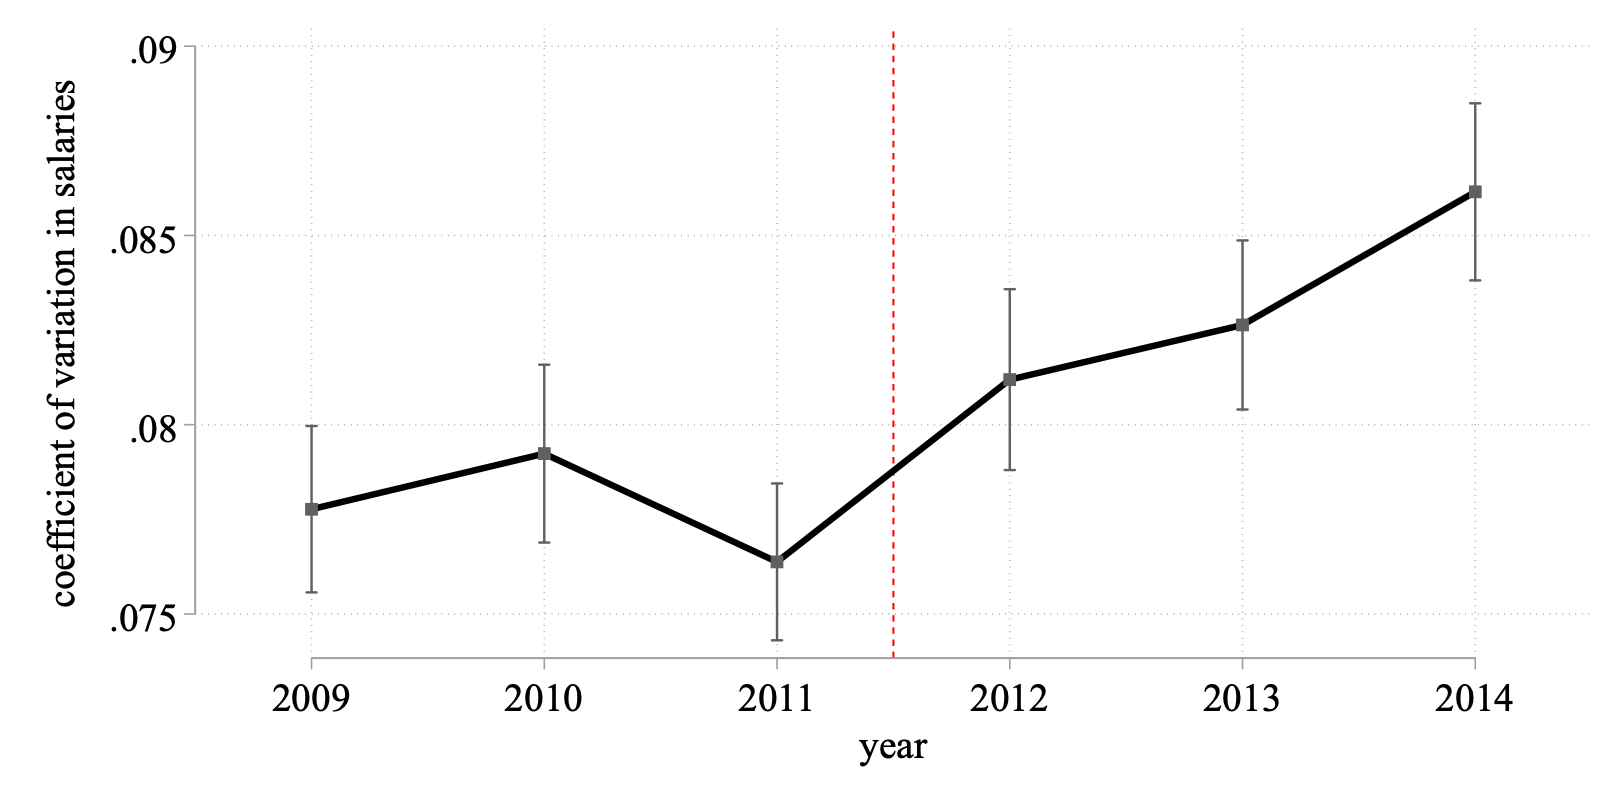
\includegraphics[width=0.9\textwidth]{figures/cvar.png}
\caption*{\footnotesize Notes: Point estimates and robust confidence intervals of the
coefficients of a regression of salary residuals on year fixed effects. Salary
residuals are obtained from a regression of salaries on district-by-year and
experience- by-years of education fixed effects.}
\vspace{-0.7cm}
\end{figure}

\noindent\textbf{Teacher Mobility:} The left panel of Figure
\ref{fig:moves} shows that movements of teachers across districts are rare,
but their frequency, i.e., the fraction of teachers employed in a district
other than the one they worked for in the previous year, more than doubled
after Act 10. The right panel shows within-teacher changes in real
wages over time, for movers and non-movers. Before Act 10, real wage growth
was small for both movers and stayers. After Act 10, wage growth remained
small for stayers but significantly increased for movers. This pattern is
consistent with districts using wage strategies to compete for teachers after
Act 10.

\begin{figure}[!ht]
\caption{Rates of Teacher Movements Across Districts}%
\label{fig:moves}
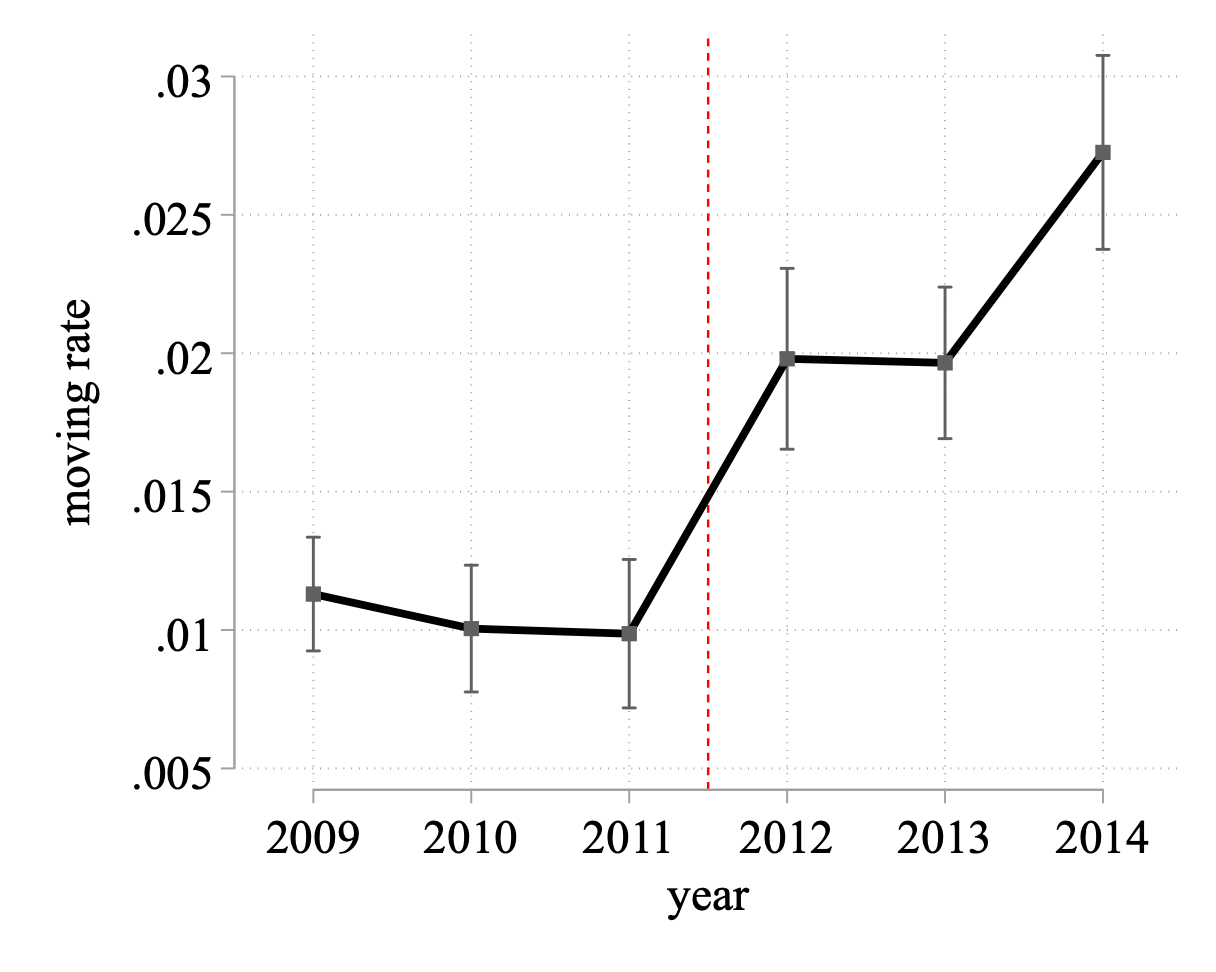
\includegraphics[width=0.49\textwidth]{figures/moves.png}
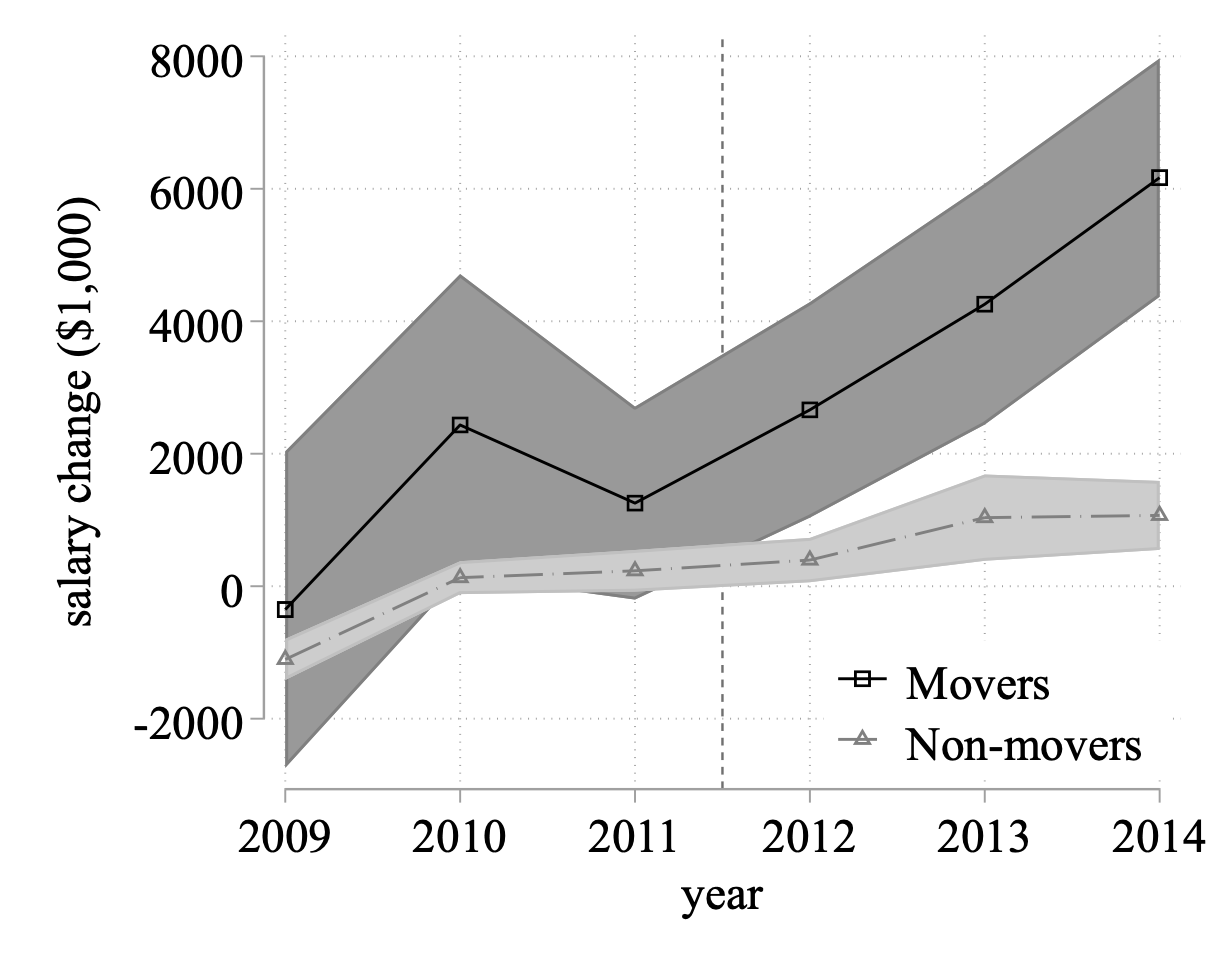
\includegraphics[width=0.49\textwidth]{figures/moving_premium_overtime.png}
\caption*{\footnotesize Notes: The left panel shows estimates and and confidence
intervals of the coefficients of a regression of an indicator for a teacher
changing district on year fixed effects, clustering standard errors at the
district level. The right panel shows estimates and confidence intervals of
year fixed effects in a regression of real salaries, where we control for
teacher fixed effects and we cluster standard errors at the district level; we
show estimates separately for movers and non-movers in each year.}
\vspace{-0.7cm}
\end{figure}

\noindent\textbf{Teacher-District Sorting:} Prior to Act 10, teachers with
higher experience, who tend to be more effective \citep{wiswall2013dynamics},
were significantly less likely to work in districts with a larger share of
low-achieving or low-SES students. Figure \ref{fig:corr} shows that the
average teacher experience of each district was negatively correlated with the
fraction of low-achieving students (those with math scores below the state
median) and the fraction of economically-disadvantaged students in the
district. These relationships became much weaker after Act 10. Before Act 10,
there was barely any (positive) correlation between average teacher experience
of each district and the district's budget; after Act 10, this correlation
became stronger. This suggests that, with the flexibility of teacher pay at
hand, districts\ with larger budgets found it even easier to attract teachers
after Act 10.

\begin{figure}[!h]
\caption{Variation in Teacher Salaries}%
\label{fig:corr}
\centering
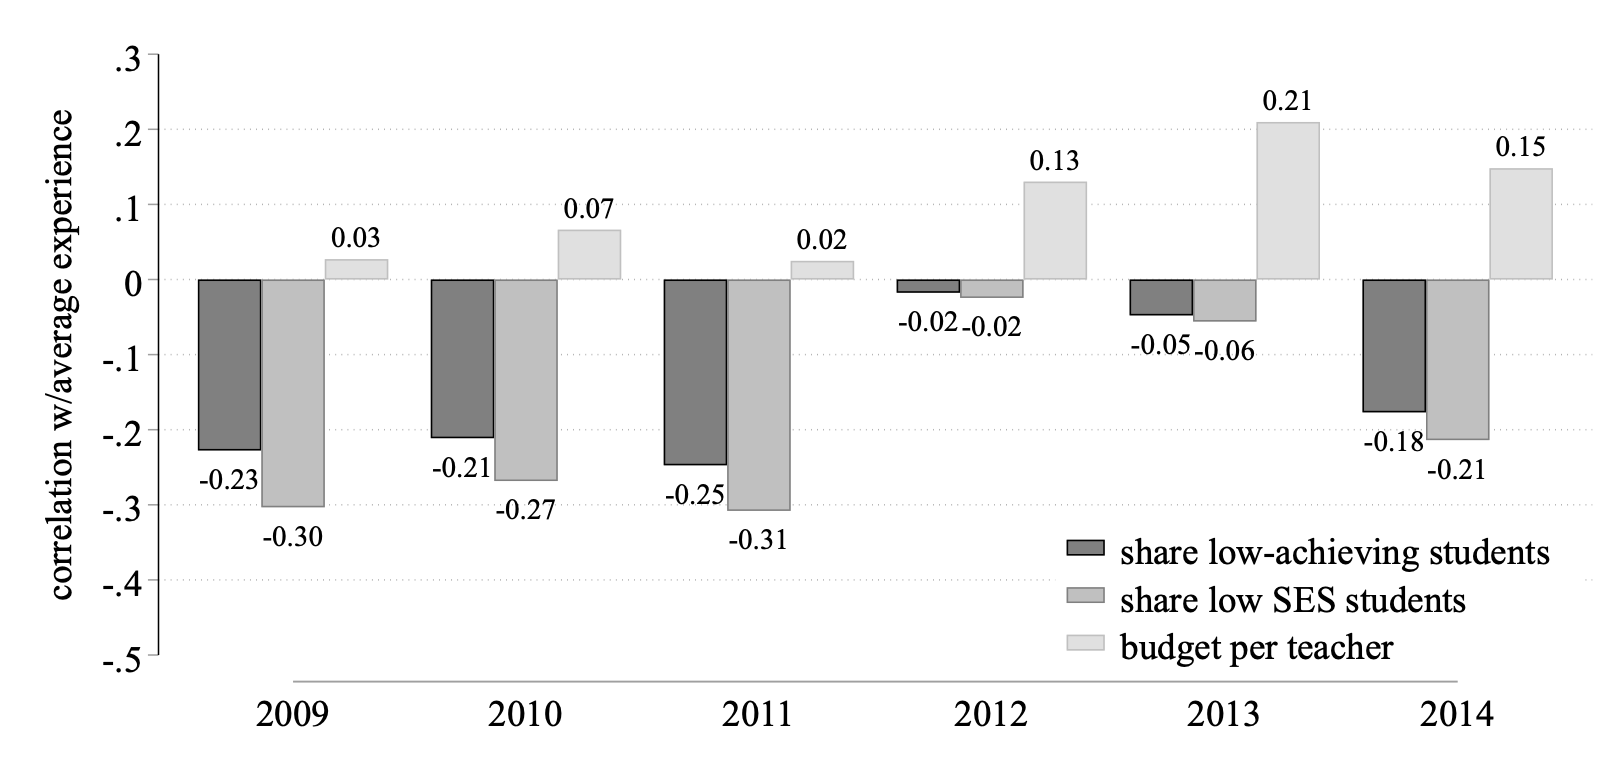
\includegraphics[width=\textwidth]{figures/sorting_correlations_lambda_overtime.png}
\caption*{\footnotesize Notes: Year-specific correlations between district
characteristics and the average experience of teachers in the district.
Correlations are obtained weighting districts by student enrollment.}%
\vspace{-0.7cm}
\end{figure}

Figures 1 to 3 provide some suggestive evidence that, under flexible pay,
districts used wage strategies to compete for teachers and teacher-district
sorting became less vertical. However, we cannot directly interpret these pre-
versus post-Act 10 differences as the effect of giving districts control over
teacher pay, because market conditions differ in other aspects between the two
eras. To isolate the equilibrium impact of replacing rigid pay with flexible
pay and, more importantly, to conduct counterfactual policy analysis, we build
the following equilibrium model.

\section{Model\label{model}}

We model a static equilibrium in the market for public school teachers, with a
distribution of teachers and $D$ school districts. Districts compete for their
preferred teachers using wage and hiring strategies; each teacher chooses
their most preferred district from those that offer them a job. Model
primitives are as follows.
\newline\textbf{Teachers: }A teacher is
characterized by $\left(  x,c,d_{0}\right)  $: The vector $x=\left[
x_{1,}x_{2}\right]  $ includes experience and education; $c=\left[
c_{1},c_{2}\right]  $ is one's effectiveness in teaching low- and
high-achieving students; $d_{0}$ is the district one works in at the beginning
of the model, where $d_{0}\in\left\{  1,...,D\right\}  $ for incumbent
teachers and $d_{0}=0$ for those who are yet to find a job on this market
(e.g., new teachers). 

It should be noted that a teacher's true effectiveness, i.e., her actual contribution to students' performance, is likely unknown to teachers and school districts, since students' performance is often measured with noise. Throughout this paper, we assume that teachers and schools observe a forecast-unbiased measure of teacher effectiveness and use it to make their decisions; we denote this measure by $c$.\footnote{Given that $c$ is forecast unbiased and enters linearly in the model we specify, using $c$ in the model is equivalent to using true effectiveness (see Section~\ref{id1} for further discussion).}  
\newline\textbf{Districts: }District $d$ is
characterized by $\left(  q_{d},\lambda_{d},\kappa_{d},M_{d}\right)  $:
$q_{d}$ is a vector of district characteristics, $\lambda_{d}$ is the fraction
of students in $d$ who are low-achieving (with prior test scores below the
state median), $\kappa_{d}$ is district $d$'s capacity (number of teaching
slots), and $M_{d}$ is its budget. The sum of slots across districts $\sum
_{d}\kappa_{d}$ is equal to the total measure of teachers in the
market.\newline A teacher's total contribution to student achievement
in district $d$\textbf{ }is given by\
\begin{equation}
TC\left(  c,\lambda_{d}\right)  \equiv\lambda_{d}c_{1}+\left(  1-\lambda
_{d}\right)  c_{2}, \label{TC1}%
\end{equation}
which, for the same teacher, varies across districts with student composition
$\lambda_{d}.$\newline\textbf{Timing: }The timing of the model is as
follows:\newline1. Districts simultaneously choose their wage schedules
$\left\{  w_{d}\left(  x,c\right)  \right\}  $ and job offers $\left\{
o_{d}\left(  x,c,d_{0}\right)  \right\}  ,$ where $o_{d}\left(  x,c,d_{0}%
\right)  =1$ if $d$ makes an offer to teacher $\left(  x,c,d_{0}\right)  $ and
$0$ otherwise. \newline2. Each teacher observes their taste shocks and chooses
their most preferred offer.

Notice that wages are assumed be blind to a teacher's origin $d_{0}$, which is
consistent with real-life practice.\footnote{Without this restriction, a
district may want to pay incumbent teachers less than non-incumbent teachers
with the same $\left(  x,c\right)  ,$ since the former are easier to attract
due to teachers' moving costs. This restriction rules out such predictions,
which are at odds with the data.} In contrast, job offers depend on $d_{0}$
because the current tenure system prevents a district from dismissing its
tenured incumbent teachers.

\subsection{Teacher's Problem}

\subsubsection{Teacher Preferences}

For a teacher with $\left(  x,c,d_{0}\right)  $, the net value of working in
$d$ is given by\newline$V_{d}\left(  x,c,d_{0}\right)  +\epsilon_{d}\equiv$%
\begin{equation}
w_{d}\left(  x,c\right)  +q_{d}\theta_{0}+\theta_{1}e^{\lambda_{d}}+\theta
_{2}\lambda_{d}c_{1}-I\left(  d\neq d_{0}\right)  \Gamma\left(  d,d_{0}%
,x_{1}\right)  +\epsilon_{d}, \label{ut1}%
\end{equation}
where\ $\epsilon_{d}$ is\ an i.i.d. Type 1 extreme-value distributed taste
shock with a scale parameter $\sigma_{\epsilon}.$ Wage enters with a
normalized coefficient of $1$, so that teachers' preferences are measured in
\$1,000. Teachers' preferences for district characteristics $q_{d}$ are
governed by the vector $\theta_{0}$. The next two terms capture teachers'
preferences for student composition $\left(  \lambda_{d}\right)  $; these
preferences may vary across teachers with different effectiveness in teaching
low-achieving students $\left(  c_{1}\right)  $.\footnote{We use
$e^{\lambda_{d}}$ in $\left(  \ref{ut1}\right)  $ because it is
disproportionately rare to see teachers move into districts with a high
fraction of low-achieving students, suggesting that teachers' preference over
$\lambda_{d}$ might be convex. We have estimated a model with $\lambda_{d}$
instead of $e^{\lambda_{d}}$; it does not fit the data well. We include only
the interaction $\lambda_{d}c_{1}$ in $\left(  \ref{ut1}\right)  $ because
adding the interaction $c_{2}\lambda_{d}$ does not improve the fit.}
$\Gamma\left(  \cdot\right)  $ is the cost of moving from $d_{0}$ to $d,$
given by
\begin{equation}
\Gamma\left(  d,d_{0},x\right)  =\left\{
\begin{array}
[c]{l}%
\delta_{0}\left(  x_{1}\right)  +\ln\left(  dist_{d,d_{0}}\right)  \delta
_{1}+I\left(  z_{d}\neq z_{d_{0}}\right)  \delta_{2}\text{ if }d_{0}%
>0\text{,}\\
\Gamma_{0}\left(  x\right)  \text{ if }d_{0}=0.
\end{array}
\right.  \label{ut2}%
\end{equation}
For teachers with $d_{0}>0,$ $\delta_{0}\left(  x_{1}\right)  $ is an
experience-group specific moving cost parameter, $\delta_{1}$ measures how
moving costs varies with (log) physical distance between two districts, and
$\delta_{2}$ is the additional cost if the new district is in a different
commuting zone than one's current district. For\ teachers new to the market
$\left(  d_{0}=0\right)  ,$ who are not attached to any district at the
beginning of the period, we assume that the moving cost from $d_{0}=0$ to any
district $d$ is the same, given by $\Gamma_{0}\left(  x\right)  $%
.\footnote{For teachers with $d_{0}=0,$ we do not observe their initial
locations. This prevents us from allowing their moving costs to differ by $d$.
Given that $\Gamma_{0}\left(  x\right)  $ is constant across districts, we set
it to zero without loss of generality because it is irrelevant for a teacher's
choice over different districts.}

\subsubsection{Teacher's Optimal Decision}

Among all received offers $\left(  o_{d}\left(  x,c,d_{0}\right)  =1\right)
$, a teacher chooses the one with the highest value:
\begin{equation}
\max_{d:o_{d}\left(  x,c,d_{0}\right)  =1}\left\{  V_{d}\left(  x,c,d_{0}%
\right)  +\epsilon_{d}\right\}  . \label{teacher}%
\end{equation}
Let $d^{\ast}\left(  x,c,d_{0},\epsilon\right)  $ be the teacher's optimal choice.

\subsection{District's Problem}

\subsubsection{District Preferences}

A teacher's (gross) value to district $d$ is given by
\begin{equation}
xb_{0}+b_{1}\lambda_{d}c_{1}+b_{2}\left(  1-\lambda_{d}\right)  c_{2},
\label{dist}%
\end{equation}
where $b_{0}$ allows for the possibility that districts may directly care
about teacher experience and education, and $b_{1}$ and $b_{2}$ capture how
much a district cares about a teacher's contribution to its low- and
high-achieving students, respectively.\footnote{Given that we only observe
accepted offers, it is hard to separate out teachers' home bias from
districts' direct preference over teachers' origins $d_{0}.$ As such, we have
assumed the latter away.} We assume that $b\geq0$, i.e., district preferences
are weakly increasing in all teacher attributes, and we normalize $b_{1}$ to
1. A special case is $b_{0}=0$ and $b_{1}=b_{2},$ in which Equation $\left(
\ref{dist}\right)  $ is equivalent to $TC\left(  c,\lambda_{d}\right)  $,
i.e., a district values a teacher only for their total contribution to its
students. More generally, if $b_{1}$ and $b_{2}$ are large relative to $b_{0}%
$, districts would rank teachers differently depending on their student
compositions $\lambda_{d};$ if $b_{0}$ is dominant, districts would largely
agree on their rankings of teachers.

\subsubsection{Choice Space for Wage Schedules}

Because wage schedules are functions, the unrestricted choice space is of
infinite dimensions. To keep the model tractable, we assume that a district's
wage schedule is a linear combination of its pre-Act 10 experience-education
wage schedule $W_{d}^{0}\left(  x\right)  $ and a teacher's contribution
$TC\left(  \cdot\right)  $:
\[
\omega_{1}W_{d}^{0}\left(  x\right)  +\omega_{2}TC\left(  c,\lambda
_{d}\right)  .\text{ }%
\]
To avoid unrealistically high or low wages, we bound wages by $\left[
\underline{w},\overline{w}\right]  ,$ such that\footnote{Empirically,
$\underline{w}$ $\left(  \overline{w}\right)  $ is 0.3 standard deviations
below (0.2 standard deviations above) the observed 1st (99th) wage percentile
in the sample.}
\begin{equation}
w_{d}\left(  x,c|\omega\right)  =\max\left\{  \min\left\{  \omega_{1}W_{d}%
^{0}\left(  x\right)  +\omega_{2}TC\left(  c,\lambda_{d}\right)  ,\overline
{w}\right\}  ,\underline{w}\right\}  . \label{wrule}%
\end{equation}
Under $\left(  \ref{wrule}\right)  ,$ a district's wage strategy boils down to
a choice of $\omega=\left(  \omega_{1},\omega_{2}\right)  \in\Omega$, where
$\Omega\subset R_{\geq0}^{2}$ is assumed to be discrete and finite.

Admittedly, the\ choice space implied by wage rule $\left(  \ref{wrule}%
\right)  $ is rather limited. However, it captures the essence of the
wage-setting problem. In particular, if $\omega=\left(  1,0\right)  \in
\Omega,$ teachers are paid on the rigid experience-education schedule, as is
the case in most U.S. school districts; if $\omega_{2}>0,$ teachers are
rewarded for their contribution, echoing the idea of performance pay. As we
show in Section \ref{wage_emp}, wages calculated under $\left(  \ref{wrule}%
\right)  $ match the observed wages very well. Appendix B1.4.3 shows
that wages predicted by three alternative and more flexible wage rules (e.g.,
rewarding $c_{1}$ and $c_{2}$ differently) are very similar to those predicted
by $\left(  \ref{wrule}\right)  $. Therefore, we choose the more parsimonious
specification $\left(  \ref{wrule}\right)  $.

\subsubsection{District's Optimal Decisions}

Taking all the other districts' policies and teachers' decision rules as
given, a district fills its capacity with its most preferred teachers by
making wage and job offer decisions, subject to its budget constraint. A
district's problem can\ be solved in two steps: First, a district chooses a
wage schedule $\omega=\left(  \omega_{1},\omega_{2}\right)  $; and second, it
makes job offers conditional on $\omega$. We solve a district's problem via
backward induction.

\paragraph{Job Offers}

For a given wage schedule $\omega$, district $d$'s job offers $\left\{
o_{d}\left(  x,c,d_{0}|\omega\right)  \right\}  _{\left(  x,c,d_{0}\right)  }$
maximize the following total value from teachers it expects to hire:\newline%
$\pi_{d}\left(  \omega\right)  =$%
\begin{align}
&  \max_{\left\{  o_{d}\left(  \cdot\right)  \right\}  }\left\{  \int
o_{d}\left(  x,c,d_{0}|\omega\right)  h_{d}\left(  x,c,d_{0},\omega\right)
\left(  xb_{0}+b_{1}\lambda_{d}c_{1}+b_{2}\left(  1-\lambda_{d}\right)
c_{2}\right)  dF\left(  x,c,d_{0}\right)  \right\} \label{pi}\\
s.t.  &  \int o_{d}\left(  x,c,d_{0}|\omega\right)  h_{d}\left(
x,c,d_{0},\omega\right)  dF\left(  x,c,d_{0}\right)  \leq\kappa_{d}%
,\nonumber\\
&  \int o_{d}\left(  x,c,d_{0}|\omega\right)  h_{d}\left(  x,c,d_{0}%
,\omega\right)  w_{d}\left(  x,c|\omega\right)  dF\left(  x,c,d_{0}\right)
\leq M_{d}\nonumber\\
&  o_{d}\left(  x,c,d_{0}|\omega\right)  =1\text{ if }x_{1}\geq3\text{ and
}d_{0}=d,\nonumber
\end{align}
where $h_{d}\left(  x,c,d_{0},\omega\right)  $ is the probability that the
teacher would accept the job \emph{if} district $d$ made them an offer
$\left(  o_{d}\left(  x,c,d_{0}|\omega\right)  =1\right)  ,$ i.e., the
probability that the teacher prefers $d$ over all the other districts that
offer them a job. Teachers' decision rule in Equation $\left(  \ref{teacher}%
\right)  $ implies
\begin{equation}
h_{d}\left(  x,c,d_{0},\omega\right)  =\frac{\exp\left(  \frac{V_{d}\left(
x,c,d_{0}\right)  }{\sigma_{\epsilon}}\right)  }{\exp\left(  \frac
{V_{d}\left(  x,c,d_{0}\right)  }{\sigma_{\epsilon}}\right)  +\sum_{d^{\prime
}\in D\backslash d}o_{d^{\prime}}\left(  x,c,d_{0}\right)  \exp\left(
\frac{V_{d^{\prime}}\left(  x,c,d_{0}\right)  }{\sigma_{\epsilon}}\right)  }.
\label{accept}%
\end{equation}
The first two constraints in $\left(  \ref{pi}\right)  $ are for capacity and
budget. The third constraint prohibits the district from dismissing\ its own
tenured incumbent teachers, as is the case in Wisconsin. Let $\left\{
o_{d}^{\ast}\left(  x,c,d_{0}|\omega\right)  \right\}  $ be the optimal job
offer decisions under wage schedule $\omega.$ Appendix A1 characterizes the
solution to $\left(  \ref{pi}\right)  $. In particular, district $d$ would
rank all teachers, except for tenured incumbents in $d\ $(because they are
already guaranteed job offers from $d$). This ranking depends only on a
teacher's value $xb_{0}+b_{1}\lambda_{d}c_{1}+b_{2}\left(  1-\lambda
_{d}\right)  c_{2}$ and wage cost $w_{d}\left(  x,c|\omega\right)  $.
Accounting for the acceptance probabilities by all teachers, including its
tenured incumbents, district $d$ would make offers to its $n$ top-ranked
teachers, where $n$ is the maximum number of offers allowed by its capacity
and budget.

\paragraph{Wage Schedule}

District $d$ chooses $\omega$ to solve the following problem%

\begin{equation}
\max_{\omega\in\Omega}\left\{  \frac{\pi_{d}\left(  \omega\right)  }%
{\kappa_{d}}-I\left(  \omega\neq\left[  1,0\right]  \right)  R_{d}\left(
\omega\right)  +\eta_{\omega}\right\}  , \label{pp}%
\end{equation}
where $\pi_{d}\left(  \omega\right)  $ (given by $\left(  \ref{pi}\right)  )$
is normalized by district capacity to make the scale comparable across
districts with different capacities$.$ Given the highly controversial nature
of Act 10, we incorporate a resistance cost $R_{d}\left(  \cdot\right)  $ that
district $d$ faces for deviating from its pre-reform wage schedule $\omega
_{d}=\left(  1,0\right)  $. Finally, $\eta_{\omega}$ is an i.i.d.
extreme-value distributed shock associated with choosing $\omega,$ with a
scale parameter $\sigma_{\eta}.$

To specify $R_{d}\left(  \cdot\right)  $ empirically, we let the institutional
background and our data guide us. As described in Section \ref{bg}, Act 10 was
a reform with political connotations: It was proposed and passed by a largely
Republican state legislature with strong opposition from Democrats, and it was
perceived by many as an attack to public-sector unions. It is therefore
plausible that districts with a larger share of Democratic voters may be more
opposed to deviating from the pre-reform rigid pay regime that is preferred by
unions. Our data support this hypothesis. As we show in Section \ref{sum},
controlling for factors that enter a district's payoff $\pi_{d}\left(
\omega\right)  ,$ the share of Democratic votes among district $d$'s residents
($dem_{d}$) is significantly negatively correlated with the deviation from the
rigid wage schedule; this correlation remains when we additionally control for
the characteristics of a district's residents.\footnote{We exclude $dem_{d}$
from teachers' preferences for parsimony: Including $dem_{d}$ in our auxiliary
regression models does not change the estimates of other coefficients nor does
it improve the $R^{2}$ of the auxiliary models, which suggests that this
variable does not explain teacher-district sorting.} We therefore allow the
resistance cost to vary with residents' political views as proxied by
$dem_{d}$ and specify $R_{d}\left(  \cdot\right)  $ as $R\left(
\omega,dem_{d}\right)  $, detailed in Appendix A2.

\subsection{Equilibrium}

\begin{definition}
\label{def}An equilibrium is a tuple of decisions $\left\{  \left\{  d^{\ast
}\left(  x,c,d_{0},\epsilon\right)  \right\}  ,\left\{  \omega_{d}^{\ast
},\left\{  o_{d}^{\ast}\left(  x,c,d_{0}|\omega\right)  \right\}  \right\}
_{d}\right\}  $ and belief $\left\{  \left\{  h_{d}^{\ast}\left(
x,c,d_{0},\omega\right)  \right\}  _{d}\right\}  $ such that\newline1) Given
$\left\{  \omega_{d}^{\ast},\left\{  o_{d}^{\ast}\left(  \cdot|\omega
_{d}^{\ast}\right)  \right\}  \right\}  _{d},$ $d^{\ast}\left(  x,c,d_{0}%
,\epsilon\right)  $ solves the teacher's problem, for all $\left(
x,c,d_{0},\epsilon\right)  $.\newline2) For all $d,$ given $\left\{
h_{d}^{\ast}\left(  \cdot\right)  \right\}  ,$ $\omega_{d}^{\ast}$ is an
optimal wage decision and $\left\{  o_{d}^{\ast}\left(  \cdot|\omega\right)
\right\}  $ are optimal job offer decisions under $\omega$.\newline3)
$\left\{  h_{d}^{\ast}\left(  \cdot\right)  \right\}  _{d}$ is consistent with
$\left\{  \left\{  d^{\ast}\left(  \cdot\right)  \right\}  ,\left\{
\omega_{d}^{\ast},\left\{  o_{d}^{\ast}\left(  \cdot|\omega_{d}^{\ast}\right)
\right\}  \right\}  _{d}\right\}  .$
\end{definition}

To solve its problem, it is sufficient for a district to know teachers'
acceptance probabilities $\left\{  h_{d}\left(  x,c,d_{0},\omega\right)
\right\}  $: Given $\left\{  h_{d}\left(  \cdot\right)  \right\}  $, knowledge
about other districts' strategies is redundant. An equilibrium requires a
consistent belief about $\left\{  h_{d}\left(  x,c,d_{0},\omega\right)
\right\}  $. However, forming the exact belief about the high-dimensional
object $\left\{  h_{d}\left(  \cdot\right)  \right\}  $ is a daunting task for
any decision maker.\footnote{The dimensionality of $\left\{  h_{d}\left(
\cdot\right)  \right\}  $ is $I\times D\times N_{w}$ ($I$, $D$ and $N_{w}$ are
the numbers of teachers, districts and potential wage levels, respectively).
Alternatively, a district can derive $\left\{  h_{d}\left(  \cdot\right)
\right\}  $ from Equation $\left(  \ref{accept}\right)  $ with its belief
about other districts' strategies. With 411 districts in the market, forming
the exact belief about other districts' wage strategies $\left\{  \left(
\omega_{d1},\omega_{d2}\right)  \right\}  $ and offer strategies is also a
daunting task.} As a feasible alternative, we assume that districts make their
decisions based on a simplified parametric belief about teachers' acceptance
probabilities,$\footnote{Similar simplification approaches have been used in
the literature to approximate equilibrium objects that are too complex to
compute exactly, e.g., \citet{lee2006intersectoral} and
\citet{meghir2015wages}.}$ given by
\begin{equation}
\widetilde{h}_{d}\left(  x,c,d_{0},\omega\right)  =\frac{1}{1+\exp\left(
f\left(  x,c,d_{0},w_{d},q_{d},\lambda_{d}\right)  \right)  }, \label{f}%
\end{equation}%
\begin{align}
f\left(  \cdot\right)   &  =x\zeta_{1}+\zeta_{2}\frac{c_{1}+c_{2}}{2}%
+\zeta_{3}\left(  \frac{w_{d}\left(  x,c|\omega\right)  -\overline{w}\left(
x,c\right)  }{\sigma_{w\left(  x,c\right)  }}\right)  +\zeta_{4}q_{d}%
+\zeta_{5}e^{\lambda_{d}}+\zeta_{6}\lambda_{d}c_{1}\label{f2}\\
&  +\left(  1-I\left(  d_{0}=0\right)  \right)  \left[  I\left(  d\neq
d_{0}\right)  \left(  \zeta_{7x_{1}}+\zeta_{8}\ln\left(  dist_{dd_{0}}\right)
+\zeta_{9}I\left(  z_{d}\neq z_{d_{0}}\right)  \right)  \right]  .\nonumber
\end{align}
This simplified belief function captures all the factors governing its
counterpart $\left\{  h_d\left(  \cdot\right)  \right\}  $ defined in $\left(
\ref{accept}\right)  $. The first two terms in $\left(  \ref{f2}\right)  $
relate to the overall desirability of the teacher: A district should expect
more competitors for a better teacher and therefore a lower acceptance
probability. The next term captures the idea that a district offering a more
competitive wage should expect a higher acceptance rate. In particular,
$\overline{w}\left(  x,c\right)  $ and $\sigma_w\left(  x,c\right)  $ are the
cross-district average and standard deviation of wages for a teacher with
attributes $\left(  x,c\right)  $, according to the wage rules chosen by all
districts in the equilibrium. We measure the competitiveness of a wage offer
$w_d\left(  x,c|\omega\right)  $ by its standardized difference from the
average $\overline{w}\left(  x,c\right)  $. The other terms in $\left(
\ref{f2}\right)  $ mirror teachers' preferences over districts'
characteristics as in $\left(  \ref{ut1}\right)  $ and moving costs as in
$\left(  \ref{ut2}\right)  $.

In the rest of the paper, we will study the market equilibrium with this
simplified belief and replace $\left\{  h_{d}\left(  x,c,d_{0},\omega\right)
\right\}  $ with $\left\{  \widetilde{h}_{d}\left(  x,c,d_{0},\omega\right)
\right\}  $ in Definition $\ref{def}.$ Solving for the equilibrium with the
simplified belief boils down to finding $\left\{  \zeta,\overline{w}\left(
\cdot\right)  ,\sigma_{w}\left(  \cdot\right)  \right\}  $ that guarantee
consistency between districts' belief $\widetilde{h}_{d}\left(  \cdot\right)
$ and teachers' acceptance rule $h\left(  \cdot\right)  $ given by Equation
$\left(  \ref{accept}\right)  $. Notice that $\left\{  \zeta,\overline
{w}\left(  \cdot\right)  ,\sigma_{w}\left(  \cdot\right)  \right\}  $ are all
equilibrium-specific and\emph{ }policy variant. For each counterfactual
policy, we will search for the associated $\left\{  \zeta,\overline{w}\left(
\cdot\right)  ,\sigma_{w}\left(  \cdot\right)  \right\}  $ that guarantee
belief consistency, using the equilibrium algorithm described in Online
Appendix B2.

\subsection{Model Discussion\label{discuss}}

For both tractability and data availability reasons, we abstract from several
important aspects. First, because we only have data within Wisconsin's public
school system, we focus on the competition among districts and abstract from
their competition against teachers' outside options (e.g., private schools,
public schools in other states, and other occupations). For the same reason,
although new teachers who ended up working in Wisconsin public schools are
included in our sample, we do not model teachers' decisions to enter or exit
the market and we take the initial distribution of teachers in the market as
pre-determined. Incorporating outside options in our framework would require
additional data and modeling decision-making by outside employers, which we
leave for future work. Some studies suggest that the effect of performance pay
on the selection into and out of the teaching profession is very small
\citep[e.g.,][]{rothstein2015teacher} and that the decision to leave teaching
is not driven by pay \citep{scafidi2006teachers}. Other studies instead
suggest that performance pay in public schools may improve the quality of the
overall supply of teachers in both public and private schools
\citep[e.g.,][]{tincani2020teacher}. If the latter is true, the efficiency
gain we find in our counterfactual policy experiments could be understated.

Second, because wage schedules are set at the district level, we focus on the
competition across districts and abstract from the allocation of teachers
across schools within a district. Appendix B3 shows that the
cross-district variation in teacher wages and student bodies clearly dominate
the within-district variation.\footnote{Of the 411 districts in Wisconsin, 173
only have one public elementary school.} Moreover, implementing the tests
proposed by \citet{chetty2014measuring} and \citet{rothstein2010teacher}, we
find no evidence of non-random sorting of teachers across grade-schools within
a district (Appendix B.3.3). That being said, focusing on
cross-district movement and competition limits our ability to conduct
counterfactual policies that introduce within-district pay variation to induce
within-district teacher reallocation. On the one hand, such policies can be
fruitful, because teachers' within-district moving costs are presumbaly lower
than their cross-district moving costs. On the other hand, districts appear to
be averse to within-district pay variation (Appendix B3); such policies
may face resistance from districts. Introducing within-district competition
and teacher reallocation into our framework would allow for a more complete
view but would involve substantial complications. We therefore leave it for
future research.

Third, we take a district's student composition $\lambda_{d}$ as given. In
particular, we assume away potential households re-sorting across districts in
response to our policy interventions. In our data, the fraction of students
moving across districts was very small and similarly so before and after Act
10; this is true for moves between any two districts and for moves between a
district that rewarded teacher effectiveness under Act 10 and one that did
not.\footnote{Between 2007 and 2016, 4.4\% of Grades 4-6 students changed
districts between two adjacent years on average. This fraction was
\emph{stable} before and after Act 10 (2011) at 4.2\% in 2010, 4.3\% in 2011,
4.2\% in 2012 and 4.3\% in 2013. Labeling districts as adopting and
non-adopting by whether or not they chose to reward teacher effectiveness
($\omega_{2}>0$ vs $\omega_{2}=0$) after Act 10, the fraction of students
moving from non-adopting districts to adopting districts was also stable at
0.8\% in 2010, 0.8\% in 2011, 0.8\% in 2012 and 0.9\% in 2013.} Our
counterfactual policies would change the baseline environment (post-Act 10
Wisconsin) only by the addition of teacher bonuses. This intervention is
milder than the introduction of Act 10 to the market. Therefore, we do not
expect our counterfactual policies to significantly affect households'
location choices. However, readers should still be aware of this limitation
when interpreting our results.

Finally, although we explicitly model how teachers' preferences,
effectiveness, opportunity sets, and hence decisions vary with their
experience, we do so in a cross-sectional reduced-form way rather than in a
life-cycle framework, with teachers internalizing their future moving costs
and job prospects. Incorporating life-cycle concerns is important but
challenging; we leave this for future work. Relatedly, we abstract from
the\ effect of financial incentives on individual teachers' effort and
effectiveness, which has been the focus of a large literature with mixed
findings.\footnote{Studies using data from outside of the US have found
evidence that financial incentives for teachers affect student achievement
\citep{muralidharan2011teacher,duflo2012incentives,lavy2002evaluating,atkinson2009evaluating,glewwe2010teacher}.
However, incentive programs implemented in the US have yielded mixed results,
e.g.,
\citet{fryer2013teacher,imberman2015incentive,dee2015incentives,brehm2017achievement}.}
We complement this literature by focusing on a different channel through which
financial incentives may improve education, i.e., by incentivizing more
efficient teacher-district matching. To the extent that teachers may improve
their effectiveness in response to financial incentives, our counterfactual
policy results could understate the total policy effects.

\section{Estimation}

We estimate the model via indirect inference using post-Act 10 data, while
holding out pre-Act 10 data for model validation. Indirect inference involves
two steps: 1) compute from the data a set of \textquotedblleft auxiliary
models\textquotedblright\ that summarize the patterns in the data; and 2)
repeatedly simulate data with the structural model, compute corresponding
auxiliary models using the simulated data, and search for model parameters
such that the auxiliary models from the simulated data match those from 1). In
particular, let $\overline{\beta}$ denote our chosen set of auxiliary model
parameters computed from the data and $\widehat{\beta}(\Theta)$ denote the
corresponding auxiliary model parameters obtained from simulating a large
dataset from the model (parameterized by $\Theta$) and computing the same
estimators. The estimated vector of structural parameters is the solution
\[
\widehat{\Theta}=\text{argmin}_{\Theta}\left\{  [\widehat{\beta}%
(\Theta)-\overline{\beta}]^{\prime}W[\widehat{\beta}(\Theta)-\overline{\beta
}]\right\}  ,
\]
where $W$ is a weighting matrix.

The estimation algorithm involves an outer loop searching for the parameter
vector $\Theta$, which consists of teachers' and districts' preference
parameters, and an inner loop solving the model for each given $\Theta$
(detailed in Appendix B2). In our counterfactual policy simulations, we
need to find the fixed point for the belief parameter vector $\zeta$
\emph{and} wage statistics $\left\{  \overline{w}\left(  \cdot\right)
,\sigma_{w}\left(  \cdot\right)  \right\}  $ that enter the belief function,
but we only need to find the fixed point for $\zeta$ during the estimation.
Assuming that the data were generated from an equilibrium, the realized
equilibrium $\left\{  \overline{w}^{o}\left(  \cdot\right)  \right\}  $ and
$\left\{  \sigma_{w}^{o}\left(  \cdot\right)  \right\}  $ can be derived
directly from the \emph{observed }wage schedules $\left\{  \omega_{d}%
^{o}\right\}  _{d}$ (the superscript $o$ denotes \textquotedblleft
observed\textquotedblright). Therefore, we can plug $\left\{  \overline{w}%
^{o}\left(  \cdot\right)  ,\sigma_{w}^{o}\left(  \cdot\right)  \right\}  $
into Equation $\left(  \ref{f2}\right)  $ and search only for the fixed point
for $\zeta$ during estimation.

\subsection{Identification}

A major identification challenge arises from the fact that, among all offers
made, the researcher observes only the accepted ones, i.e., the realized
teacher-district matches. This makes it hard to separate teachers' preferences
from districts' preferences
\citep[see, for example,][]{menzel2015large}.\footnote{In the setting of
two-sided matching markets with non-transferable utility,
\citet{menzel2015large} shows that, under pairwise stable matching, the joint
surplus is non-parametrically identified and that, without further
assumptions, it is impossible to identify preferences on each side of the
market separately. \citet{ederer2023labor} extends \citet{menzel2015large} to
a dynamic setting.} Some studies tackle this challenge using data on teachers' job applications \citep{bates2022teacher} or schools' rankings of
teachers \citep{ederer2023labor}. Other rely on instrumental variables that
affect one side's payoffs but are excluded from the other side's preferences \citep{agarwal2015empirical,laverde2025gains}.\footnote{In a
centralized student-school matching system, \citet{fack2019beyond} define a
student's feasible choice set as the set of schools whose observed ex post
admission cutoffs are below the student's priority index; they estimate
students' preferences assuming stability.} We take a different approach: As we argue below, the observed wage schedules and matches contain rich information that allows us to overcome this identification challenge under an assumption of information symmetry between the district and the researcher. This argument guides our choice of auxiliary models.

\subsubsection{Wage Schedule and District Pre-Determined Conditions\label{id2}%
}

Under Act 10, districts can choose how to reward teachers. Therefore, the
observed wage schedules provide the first major source of information for
identification: One can learn about districts' preferences from the extent to
which their wage schedules favor teachers with different attributes $\left(
x,c\right)  $ and how wage schedules relate to districts' pre-determined
conditions. To see the intuition, it is useful to notice that wage schedules
can serve to both pull and push teachers. To pull teachers with its preferred
attributes $\left(  x,c\right)  ,$ a district should choose a wage schedule
that favors $\left(  x,c\right)  $. The need to do so is stronger when these
teachers are not district incumbents, because moving is costly for teachers.
Meanwhile, although a district cannot dismiss its tenured incumbents with
undesirable $\left(  x^{\prime},c^{\prime}\right)  $, it can push them out by
choosing a wage schedule that disfavors $\left(  x^{\prime},c^{\prime}\right)
$. Notice that district $d$ can avoid teachers with $\left(  x^{\prime
},c^{\prime}\right)  $ who are not $d$'s tenured incumbents simply by not
offering them jobs. Therefore, the incentive to use a wage schedule
disfavoring $\left(  x^{\prime},c^{\prime}\right)  $ is stronger if the
district has more tenured incumbents with $\left(  x^{\prime},c^{\prime
}\right)  .$

However, district preferences over teachers may not be sufficient to explain
the observed wage schedule choices. For example, in our post-Act 10 data, 24\%
of districts kept their pre-Act 10 wage schedules and 50\% of districts\ chose
not to reward teacher effectiveness. It is hard to rationalize these mass
points as optimal wage schedules chosen by districts purely to hire their
preferred teachers. Districts' choices that are not explained by their
preferences for teachers are attributed to the resistance cost $R\left(
\cdot\right)  .$

\subsubsection{Optimal Job Offers and Observed Matches\label{id1}}

The observed teacher-district matches provide the second major source of
information for identification. If we observed each teacher's feasible options, we could identify teachers' preferences in a straightforward
way: choices out of\ (multiple) feasible options reveal preferences. Observing
only accepted offers complicates the inference.

However, combining the observed matches with districts' optimal offer
decisions allows us to infer a subset of all offers received by each teacher
and thus to identify teachers' preferences. Specifically, for district $d,$
the marginal benefit of hiring a teacher consists of the teacher's
contribution to district $d$'s low-achieving students $\lambda_{d}c_{1}$ and
high-achieving students $\left(  1-\lambda_{d}\right)  c_{2},$ and the direct
value of their experience and education $x.$ The marginal cost consists of
teacher wage $w_{d}\left(  x,c|\omega_{d}^{o}\right)  $ (calculated using wage
rule $\left(  \ref{wrule}\right)  $ at the observed schedule $\omega_{d}^{o}$)
plus the shadow price of a slot. If $d$ hires a teacher $i$ who is not a
tenured incumbent in $d$ (which implies that the offer is based on $d$'s
preference rather than on the non-dismissal constraint), then for any district
preference parameter vector $b\geq0,$ a teacher $j$ is at least as preferable
as $i$ and hence must also receive an offer from $d$ if the following
(sufficient but not necessary) conditions are met: 1) $j$ has weakly higher
$c_{1},$ $c_{2}$ and $x$ than $i,$\footnote{We assume that teacher experience
$\left(  x_{1}\right)  $ enters district preferences as ordered categorical
variables (0-2, 3-4, 5-9, 10-14, 15 years or more). Therefore, the comparison
of teacher experience $\left(  x_{1}\right)  $ is based on these categories.}
and 2) $w_{d}\left(  x_{j},c_{j}|\omega_{d}^{o}\right)  \leq w_{d}\left(
x_{i},c_{i}|\omega_{d}^{o}\right)  $. With this argument, we can use observed
matches ($\left(  i,d\right)  $ in this example) to infer offers for other
teachers ($j$ in the example). Then, for each teacher $i$, we can construct
(observe) a subset $O_{i}^{s}$ of all the offers they received, consisting of
the inferred offers, the accepted offer, and, if $i$ is tenured, the
guaranteed offer from $i$'s original employer $d_{0i}$. Given the assumption
that $b\geq0,$ all options in $O_{i}^{s}$ are offered to teacher $i$,
therefore as long as $O_{i}^{s}$ is not a singleton (which is true for 5,170
out\ of 6,600 teachers in our sample) a teacher's choice within (the observed)
$O_{i}^{s}$ identifies their preferences--- how much teachers value districts'
characteristics relative to wages and how dispersed their preference shocks
are.\footnote{Multinomial discrete-choice models can be point-identified using
a subset of choices, parametrically \citep[e.g.,][]{mcfadden1977modelling} and
semiparametrically \citep[e.g.,][]{fox2007semiparametric}. In a framework much
more flexible than ours, \citet{barseghyan2021heterogeneous} allow for
\emph{unrestricted correlation} between choice sets and preferences and
characterize the sharp identification region of model parameters. We build on
insights from these studies to design our auxiliary model Aux 1a (Section
\ref{aux}), which is used to extract information useful for identification.}

Observed matches are also informative of district preferences. First, as the
number of teachers per district grows large, the lowest $\left(  x,c\right)  $
among teachers working in $d$ is the lowest $\left(  x,c\right)  $ that
district $d$ is willing to hire. This is because teachers are subject to
preference shocks with an unbounded support and an offer would be accepted by
some teacher. The lowest $\left(  x,c\right)  $ within each district
identifies districts' preferences over teachers.

In practice, many districts are small, therefore, our identification also
relies on the following observation. Given that the distribution of teachers'
preferences is revealed from their choices within $O_{i}^{s}$,\ we can predict
the probability that a teacher would choose to work in each district if they
had offers from \emph{all districts.} As long as at least some districts are
selective (i.e., they do not make offers to all teachers), accounting for
teacher preference shocks, this predicted distribution of teacher-district
matches will be systematically different from the observed matches, because a
teacher can choose a district $d$ only if they have an offer from $d.\ $That
is, given teachers' preferences, districts' offer decisions---which are
governed by districts' preferences---must rationalize the realized match distribution.

The identification argument can be illustrated with a simple example (see
Appendix B4.3 for a graphical illustration). Consider the simpler case
where teachers do not have preference shocks and suppose that two teachers $i$
and $j$ both prefer district $1$ over district $2$. If we observe $i$ working
in district $1$ and $j$ working in district $2$, it must be the case that
district $1$ prefers $i$ over $j.$ The same argument applies when teachers
have preference shocks: If teachers systematically prefer district $1$ over
district $2$, then district $1$ must prefer their hires over (most) teachers
working in district $2.$ As long as the distribution of $\left(  x,c\right)  $
in district $1$ does not systematically dominate the distribution of $\left(
x,c\right)  $ in district $2$ in all dimensions, we can infer how much
district $1$ cares about $x$ and $c_{2}$ relative to $c_{1}$ (the coefficient
for $c_{1}$ is normalized to $1$).

\paragraph{Discussion}

Our strategy of identification using realized matches contains three
steps. To better understand our strategy, we highlight, step by step, which assumptions are necessary and which are made for convenience.


\noindent \textbf{Step 1:} We construct subsets of offers faced by each teacher, under two types of assumptions. The first is that districts and the researcher share the same
information about teacher effectiveness (or more generally, teacher traits
that enter districts' payoff function), which involves A1 and A2 below. The second type of assumption relates to job posting and job application (A3 below). Notice that the specific functional form of $B\left(
\cdot\right)  $ is irrelevant here as long as $B\left(  \cdot\right)  $ is
weakly increasing in every dimension of teacher trait. Moreover, as long as
the researcher observes the same measures of teacher traits as districts do, be them exact or noisy measures, our estimation strategy, estimates, and policy implications on expected outcomes remain the same (see Online Appendix B4.1 for further discussion). %\ In particular, although we label $c$ as teachers' effectiveness, $c$ is an estimate rather than the true measure (which may not be observed by anyone). The key assumption is that districts use $c$ to make their decisions. 
More specifically, we rely on the following assumptions. 


\noindent \textbf{A1}: $\left(  x,c\right)  $ are observable to
all districts; in particular, districts and the researcher share the same information about teachers' effectiveness, i.e., the forecast-unbiased measure estimated from the test score data.\footnote{\citet{jacob2008can} find that principals can
generally identify very effective and very ineffective teachers but are less
able to distinguish between teachers in the middle of the effectiveness
distribution.} As a robustness check, we conduct the following exercise in Online
Appendix B4: Instead of $\left(  c_{1},c_{2}\right)  ,$ districts observe
$\left(  c_{1}+err_{1},c_{2}+err_{2}\right)  $ and make wage and job offer
decisions based on these noisy measures. Assuming that $err_{k}$ are i.i.d.,
normally distributed noise terms for $k=1,2$, we repeat the procedure
described in Section $\ref{id1}$ to construct subsets of offers for each
teacher and re-estimate our key auxiliary models that summarize teachers'
choices within these subsets. These auxiliary models are robust to this simple
form of information friction.

\noindent \textbf{A2}: Districts cannot discriminate among
teachers by factors other than $\left(  x,c\right)  $. If some job offers were
made for reasons other than $\left(  x,c\right)  $, then the inferred
$O_{i}^{s}$ might include infeasible options for some teachers and thus
introduce bias in the inferred teacher preferences based on $O_{i}^{s}.$
However, as long as most job offers are based on $\left(  x,c\right)  $, the
essence of our identification strategy still holds: Teacher preferences
inferred from $O_{i}^{s}$ would still be much closer to their true preferences
than those inferred assuming that teachers had offers from all districts. As a
robustness check, in Appendix B4, we re-estimate our key auxiliary
models but do not use observed teacher-district $\left(  i,d\right)  $ matches
to infer offers for other teachers if $i$'s effectiveness (either $c_{1}$ or
$c_{2}$) is below the 10th percentile among all teachers, since these
ineffective teachers may indeed have been hired for other reasons. Doing so
significantly affects the number of inferred offers for other teachers; yet
our auxiliary models remain robust. 

\noindent \textbf{A3}: The cost of posting jobs is zero. This assumption is plausible because in reality districts post openings
publicly on online platforms.\footnote{See, e.g.,
https://wecan.education.wisc.edu (Wisconsin Education Career Access Network).}
We also assume that teachers get offers without having to apply. This
assumption does not affect our inference of teacher preferences because the
following two cases would both imply that district $d$ was not attractive
enough to teacher $j:$ 1) $d$ made an offer to $j$ and $j$ did not accept it;
2) $j$ was eligible for a job in $d$ but did not apply. If it is costly for
teachers to apply for jobs (more so for jobs in districts other than one's
initial district), then these costs would be absorbed in teachers' moving
costs in our model.\\

\noindent \textbf{Step 2: } We identify teachers'
preferences from their choices within the inferred subset of offers, following  Fox (2007), who proves semiparametric identification of multinomial discrete-choice models using a subset of options. Besides standard
regularity conditions, the identification relies on two conditions. The first
condition is rank-ordering: Choices with higher deterministic payoffs are more
likely to be chosen by a given agent. The second condition is exchangeability,
also known as label independence. These two conditions hold in a large set of
multinomial discrete-choice models (with additively-separable error terms),
including ours.\footnote{The first condition requires that for a given agent,
choice probabilities are rank ordered by deterministic payoffs (random
coefficient models violate this condition), but two agents with only slightly
different deterministic payoffs can make choices with different probabilities.
The second condition holds for any collection of i.i.d. random variables.}
Provided that preference shocks are additively separable, specific
distributional assumptions are not necessary; we assume Type-1 extreme-value
distribution for convenience. These arguments hold for teachers with at least
two offers in $O_{i}^{s}$; we rely on extrapolation to identify preferences
for other teachers.\footnote{Teachers with only 1 offer in $O_{i}^{s}$ are less experienced, less effective, but more educated (Appendix Table B13).}\\

\noindent\textbf{Step 3: } Given teachers' preferences, we identify districts'
preferences. Unlike the teacher-side of the problem, we know each
district's choice set---the entire sample of teachers. Given A1-A3, as long as a district
does not make offers to all teachers, its preference is revealed by its offer decisions. Moreover, provided that districts agree that teacher $i$ is weakly better than $j$ if $i$ has higher $\left(  x,c_{1},c_{2}\right)  ,$ we can allow districts
to differ in how they rank teachers in ways that are more flexible than our
current (parsimonious) specification.\footnote{For example, we can allow for any interaction of teachers' and districts' traits, provided that $B(.)$ is weakly increasing in teacher traits.}

\subsection{Auxiliary Models\label{aux}}

The identification argument in Section $\ref{id2}$ suggests targeting
statistics on the relationship between districts' wage schedules and their
pre-determined conditions; the argument in Section $\ref{id1}$ suggests
targeting statistics that summarize 1) teachers' choices within the inferred
offer subset $O_{i}^{s}$ and 2) the realized distribution of teacher-district
matches. Although certain auxiliary models are intuitively more informative
about certain structural parameters than others (as we explained above), the
identification of the model relies on using information extracted from
\emph{all} auxiliary models. Therefore, we target the following auxiliary
models\emph{ jointly}. To provide more evidence on the mapping between data
and parameters, in Appendix B5 we follow \citet{einav2018provider} and
perturb structural parameters one by one, measuring the responses of the
predicted auxiliary models.

\begin{enumerate}
\item[Aux 1] Coefficients from two regressions of the form%
\[
y_{id}=\beta_{1}^{m}w_{id}+I\left(
\begin{array}
[c]{c}%
d_{0i}>0,\\
d\neq d_{0i}%
\end{array}
\right)  \left[
\begin{array}
[c]{c}%
\beta_{2}^{m}\left(  x_{i1}\right)  +\beta_{3}^{m}\ln\left(  dist_{id}\right)
\\
+\beta_{4}^{m}I\left(  z_{d}\neq z_{d_{0i}}\right)
\end{array}
\right]  +q_{d}\beta_{4}^{m}+\beta_{5}^{m}e^{{\small \lambda}_{d}}+\beta
_{6}^{m}c_{1i}\lambda_{d}+\psi_{i}+\varepsilon_{id}^{m},
\]
where $y_{id}=1$ if teacher $i$ is matched with district $d,$ and $0$
otherwise. The right-hand-side variables are the same as those entering
teachers' preferences, including $w_{id}\equiv w\left(  x_{i},c_{i}|\omega
_{d}\right)  ,$ the wage $i$ would be paid by district $d$ under wage rule
$\left(  \ref{wrule}\right)  $. $\psi_{i}$ is a teacher dummy that relates all
$\left\{  \left(  i,d\right)  \right\}  _{d}$ observations associated with
teacher $i$.\footnote{Although conditional logit regressions would be a more
intuitive way to summarize discrete choices, they are computationally too
costly to run during the estimation. We\ instead use a linear regression with
teacher fixed effects. These fixed effects (not targeted) serve to capture the
idea that the same teacher is choosing one district out of a given set of
districts.} The two regressions differ in the number of observations,
reflecting the argument in Section $\ref{id1}.$

\begin{enumerate}
\item[Aux 1a] The first regression includes all teachers whose inferred
subsets $O_{i}^{s}$ contain more than one offer; an observation $(i,d)$ is a
teacher-district pair in these inferred subsets.

\item[Aux 1b] The second regression includes every possible teacher-district
pair, which serves to summarize observed teacher-district matches.
\end{enumerate}

\item[Aux 2] Moments of district-level teacher characteristics $\left(
x,c_{1},c_{2}\right)  $ by district groups (quintiles of $\lambda_{d},$
quintiles of budget per slot, and urban/suburban status), which supplement Aux 1b.

\item[Aux 3] \label{aux3}Coefficients from regressions of wage schedule
$\omega_{dn},$ $n=1,2$, on district's pre-determined conditions, reflecting
the identification argument in Section $\ref{id2}$:%
\begin{align*}
\omega_{dn}  &  =\beta_{0n}^{w}+q_{d}\beta_{1n}^{w}+\beta_{2n}^{w}\lambda
_{d}+\beta_{3n}^{w}\kappa_{d}+\beta_{4n}^{w}M_{d}+X_{d}\beta_{5n}^{w}%
+\beta_{6n}^{w}\overline{TC}_{d}+\beta_{7n}^{w}\overline{TC}_{d}^{tenure}\\
&  +\beta_{8n}^{w}\overline{TC}_{z_{d}}+\beta_{9n}^{w}\overline{Tenured}%
_{z_{d}}+\beta_{10n}^{w}dem_{d}+\varepsilon_{dn}^{w},
\end{align*}
where coefficients $\beta_{1n}^{w}$ to $\beta_{4n}^{w}$ are associated with
district characteristics and constraints, and $\beta_{5n}^{w}$ to $\beta
_{7n}^{w}$ are associated with the composition of district incumbents. In
particular, $X_{d}$ is the average $x,$ $\overline{TC}_{d}$ is the average
$TC$ among teachers with $d_{0i}=d$, and $\overline{TC}_{d}^{tenure}$ is the
average $TC$ among the district's tenured incumbents $\left(  d_{0i}=d\text{
and }x_{1i}\geq3\right)  $. The next two terms are about teachers originally
working in other districts within $d$'s commuting zone (i.e., $d_{0i}\neq d,$
but $z_{d_{0i}}=z_{d}$): their average TC ($\overline{TC}_{z_{d}}$) and
tenured rate ($\overline{Tenured}_{z_{d}}$). Lastly, $dem_{d}$ is the share of
Democratic votes in the district.

\item[Aux 4] Cross-district wage schedule moments, which supplement Aux 3:
$E\left(  \omega_{1}\right)  ,$ $E\left(  \omega_{2}\right)  ,$ $E\left(
\omega_{1}^{2}\right)  ,$ $E\left(  \omega_{2}^{2}\right)  ,$ $E\left(
\omega_{1}\omega_{2}\right)  ,$ $E\left(  \omega=\left(  1,0\right)  \right)
$, $E\left(  \omega_{1}dem\right)  ,$ and $E\left(  \omega_{2}dem\right)  .$
\end{enumerate}

\section{Data\label{data}}

Our data, from the Wisconsin Department of Public Instruction (WDPI), consist
of three linked data sets that provide information about teachers, students,
and districts respectively. All of our data are reported by academic year and
referenced by the calendar year of the spring semester (e.g. 2014 for the
2013-14 academic year).

\medskip\noindent\textit{\textbf{Teacher-Level Data}} \citep[PI-1202 Fall Staff
Report][]{wdpi_admin_2006_2016} cover all individuals employed by the WDPI between 2006 and 2016. This
panel provides information about teachers' education, years of teaching
experience, total wages, full-time equivalency units, school and district
identifiers, and grades and subjects taught.

\nocite{wdpi_cesa}
\nocite{wdpi_school_districts_2024}
\nocite{nces_school_district_boundaries}
\nocite{bergeron_etal_2022_life_expectancy_data}
\nocite{dailykos_county_cd_overlaps_117}
\nocite{google_maps_2022}

\medskip\noindent\textit{\textbf{Student-Level Data }}include demographics and
state standardized test scores for all public school students in Grades 3 to 8
between 2007 and 2016.

\medskip\noindent\textit{\textbf{District-level Information: }}Using student
test score data, we calculate $\lambda_{d}$, the fraction of students in
district $d$ whose prior math scores were below the grade-specific state
median. District characteristics $q_{d}$ include indicators for urbanicity
(urban, suburban or rural) and for being in a large metropolitan area, all
based on the 2010 Census classification. Each district is assigned to one of
19 commuting zones $z_{d}$.

\subsection{Empirical Definitions}

To map our equilibrium model to the data, we use the following empirical
definitions (more details are in Appendix B1).

\subsubsection{The Market\label{market}}

Our model is in a static equilibrium setting. For estimation and
counterfactual policy analyses, we use data from 2014, i.e., 3 years after Act
10; by then, all the CB agreements pre-dating Act 10 had expired and districts
had obtained full autonomy over teacher pay.\footnote{\citet{biasi2018labor}
shows that teacher exits surged in 2012 but had stabilized by 2014.} To
validate the estimated model, we simulate the market equilibrium under rigid
pay and initial conditions in 2010 data, i.e., the year preceding Act 10.

In both years, we focus on the market for non-substitute full-time public
school math teachers in Grades 4-6, for the following reasons. We exclude the
few substitute and part-time teachers because they face different types of
contracts than regular, full-time teachers.\footnote{Among all public school
teachers teaching Grades 4-6 math in 2014 (2010), 2.0\% (1.8\%) were
substitute teachers and 2.8\% (3.9\%) were part-time teachers.} We exclude
secondary-school teachers because they often teach multiple grades, making it
hard to identify individual teacher contributions
\citep{kane2008estimating,chetty2014measuring}. Among elementary-school
teachers, we focus on those for whom we can construct effectiveness measures,
i.e., teachers in Grades 4-6. We further restrict attention to teachers of the
same subject (math), so that the effectiveness measures are comparable across
teachers.\footnote{The achievement models used to calculate teachers'
effectiveness include students' lagged test scores; since students are tested
starting from Grade 3, we can only calculate teacher effectiveness starting
from Grade 4. We choose math over English because previous studies have found
that teacher effects on students are larger in math than in reading or
language
\citep[e.g. ][]{rivkin2005teachers,kane2008estimating,chetty2014measuring}.
Appendix Figure B7 shows that the fraction of teachers switching into
or out of math was very small in the data and the frequency did not change
after Act 10. Therefore, we take the distribution of teachers across math and
non-math subjects as given and our counterfactual analysis abstracts away from
potential policy effects on teachers' sorting across subjects.} The estimation
sample contains 411 districts and 6,600 teachers; the validation sample
contains 411 districts and 6,741 teachers.

By focusing on a subgroup of teachers, we have implicitly assumed that a
district's capacity and budget constraints for this subgroup do not interact
with those for other teachers. This assumption will hold if, for example, a
district commits certain resources for the math education of its Grade 4-6
students. Appendix Figure B8 supports this hypothesis: The share of a
district's budget spent on Grade 4-6 math teachers is stable over time.

\subsubsection{Teacher Characteristics\label{teacherX}}

\medskip\noindent\textit{\textbf{Teacher Effectiveness: }}$c_{i1}$ and
$c_{i2}$ are $i$'s contributions to the achievement of low- and high-achieving
students, respectively.\textit{\textbf{ }}To obtain $\left(  c_{i1}%
,c_{i2}\right)  $ for each $i$, we modify the student achievement model in
\citet{kane2008estimating} to allow for two-dimensional effectiveness as
follows:
\begin{equation}
A_{kt}=\gamma Z_{kt}^{s}+\sum_{i:SG_{kt}=SG_{it}^{T}}\left(
\begin{array}
[c]{c}%
I\left(  \tau_{k}=1\right)  (\rho_{1}x_{it}+v_{i1})\\
+I\left(  \tau_{k}=2\right)  (\rho_{2}x_{it}+v_{i2})
\end{array}
\right)  +\varepsilon_{kt}, \label{achievement}%
\end{equation}
where $A_{kt}$ is student $k$'s achievement (standardized math score) in year
$t$; $Z_{kt}^{s}$ includes a vector of student observables (including
$A_{kt-1})$, a school-grade fixed effect, and a year fixed effect;
$\varepsilon_{kt}$ is an i.i.d. idiosyncratic component. In the summation,
$SG_{kt}$ ($SG_{it}^{T})$ denotes the school-grade student $k$ (teacher $i)$
belongs to in year $t$; $\tau_{k}$ denotes a student's type ($\tau_{k}=1$ if
$k$ is low-achieving, i.e., if $k$'s prior score is below the grade-specific
state median; $\tau_{k}=2$ if $k$ is high-achieving). For a student of
achievement type $n\in\left\{  1,2\right\}  ,$ teacher $i$'s contribution is
given by $\rho_{n}x_{it}+v_{in},$ where $x_{it}$ denotes $i$'s education and
experience in year $t$ and $v_{in}$ is the part unexplained by $x_{it}.$
Assuming that student-teacher sorting is random across school-grades
conditional on observables, we estimate $\gamma$, $\rho_{1}$ and $\rho_{2}$
via OLS using data from 2007 to 2016; then, we use the Bayes estimator of
\citet{kane2008estimating} to estimate $v_{i1}$ and $v_{i2}$, which are forecast unbiased (Appendix
B1.3.1). Finally, we construct teacher effectiveness $\left(  c_{i1}%
,c_{i2}\right)  $ in our model as
\begin{equation}
c_{in}\equiv\widehat{\rho}_{n}x_{it^{\ast}}+\widehat{v}_{in},\ n\in\{1,2\},
\label{cc}%
\end{equation}
where $t^{\ast}$ is 2014 for the estimation sample and 2010 for the validation
sample.\footnote{Following the literature, we measure $c_{i1}$ and $c_{i2}$ as
residual contributions to standardized test scores; given that the mean of
test scores is 0, $c_{i1}$ and $c_{i2}$ can be negative. In order to make sure
that all teachers have a (weakly) positive contribution to a district's
objective value $\left(  \ref{pi}\right)  $ and that a district would not want
to leave classrooms unstaffed, we replace $c_{1}$ and $c_{2}$ in $\left(
\ref{pi}\right)  $ with $\left(  c_{1}-\underline{c}_{1}\right)  $ and
$\left(  c_{2}-\underline{c}_{2}\right)  ,$ where $\underline{c}_{1}$
($\underline{c}_{2}$) is the minimum of $c_{1}$ ($c_{2})$ across all teachers
in the sample. Notice that this re-scaling is innocuous because it does not
affect how a district ranks teachers.}

Two features of our achievement model deserve further discussion. First, we
focus on teachers' comparative advantages in terms of $\left(  c_{1}%
,c_{2}\right)  $ because our two-dimensional effectiveness model explains
approximately 20\% more variation in test scores compared to the
one-dimensional effectiveness model (Appendix B1.3.4). In contrast, if
we add, for example, a teacher's race and its interaction with student race to
the achievement model, the interaction terms are indistinguishable from zero
(Appendix B1.3.5).

Second, besides modeling $c$ as being two-dimensional, we also allow $c$ to
vary directly with $x,$ because experience has been shown to affect teacher
effectiveness \citep[e.g.,][]{rockoff2004impact,wiswall2013dynamics}. To
estimate effectiveness with this feature, we have to assume that a teacher
contributes to all students in their school-grade in $\left(
\ref{achievement}\right)  $ because we can link students and teachers only up
to the school-grade level. In an alternative model where a teacher contributes
only to students in their class, we can use our data to identify teacher
effectiveness assuming that it is invariant to one's experience.
Identification of both models exploits teacher turnover across school-grades
and the assumption that $\varepsilon_{kt}$ and $v_{in}$ are uncorrelated.
Notice that this assumption allows for endogeneous district-teacher sorting
(as is the case in our model), because we control for $Z_{kt}^{s}$, which
includes school-grade fixed effects and year fixed effects. As we show in
Appendix B1.3.3, the estimated teacher effectiveness measures from the
two achievement models are highly correlated; more importantly, auxiliary
models Aux 1a and 1b, which provide key information for the identification of
our equilibrium model, are very similar using either type of effectiveness
measures. In addition, the precision of our effectiveness measures is
comparable with that of measures from studies using teacher-classroom linked
data. That said, since teacher effectiveness is estimated with noise,
our counterfactual policy implications should be interpreted with due caveat.\footnote{Relatedly, given that less experienced teachers are observed for fewer years, their estimated effectiveness is noisier and hence shrunk more toward zero in our estimation procedure.} 

\medskip\noindent\textit{\textbf{Teacher's Origin District}}: For the
estimation sample, we use teachers' employment histories between 2011 (when
Act 10 was passed) and 2014 and define $d_{0i}$ as $i$'s last employer before
2014. We follow the same procedure for the validation sample, using a
teacher's employment history between 2007 and 2010.

\subsubsection{Wage Schedules and District Constraints\label{wage_emp}}

\medskip\noindent\textit{\textbf{Pre-Act 10 Wage Schedules }}$\left\{
W_{d}^{0}\left(  x_{i}\right)  \right\}  _{d}$ are obtained using data from
2007 to 2011. Specifically, $W_{d}^{0}\left(  x_{i}\right)  $ is the predicted
value from a regression of observed pre-Act 10 teacher real wages (in 2014
dollars) on indicators for experience groups and education groups, where the
regression coefficients are allowed to differ across districts$.$

\medskip\noindent\textit{\textbf{Choice Set for Wage Schedules }}$\left(
\Omega\right)  $\textbf{: }We first construct a grid $\Omega^{o}$ such that
wages $w_{d}\left(  x_{i},c_{i}|\omega\right)  $ under $\left(  \ref{wrule}%
\right)  $ and $\omega\in\Omega^{o}$ provide a good coverage of the observed
wage distribution. We then expand the grid range, such that the model choice
set $\Omega\supset\Omega^{o}$, to allow for the possibility that district
choices may go out of the empirical range in counterfactual scenarios. We use
the same $\Omega=\left\{  0.9,0.95,1,1.05,1.1,1.15\right\}  \times\left\{
0,10,30,50,75,100,200,225\right\}  $ throughout.

\medskip\noindent\textit{\textbf{District Wage Schedules}}: For each district,
we find the grid point on $\Omega$ that best summarizes the observed wages
$\left(  w_{i}^{o}\right)  $ of teachers working in $d$ $\left(
d(i)=d\right)  $:
\[
(\omega_{d1}^{o},\omega_{d2}^{o})=\arg\min_{(\omega_{1},\omega_{2})\in\Omega
}\sum_{i:d(i)=d}\left(  w_{i}^{o}-w_{d}\left(  x_{i},c_{i}|\omega\right)
\right)  ^{2},
\]
where $w_{d}\left(  x_{i},c_{i}|\omega\right)  $ is given by wage rule
$\left(  \ref{wrule}\right)  ;$ $\left(  \omega_{d1}^{o},\omega_{d2}%
^{o}\right)  $ is treated as district $d$'s wage schedule in the realized
equilibrium. The implied $\left\{  w_{d}\left(  x_{i},c_{i}|\omega_{d}%
^{o}\right)  \right\}  $ matches the data $\left\{  w_{i}^{o}\right\}  _{i}$
very well.\footnote{The estimated slope coefficient of a linear model of
$w_{i}^{o}$ as a function of $w_{d}\left(  x_{i},c_{i}|\omega_{d}^{o}\right)
$ equals 0.88 (with a standard error of 0.004) and an $R^{2}$ of 0.85.
Focusing on the subsample of movers, the estimated slope coefficient is 1.08,
with a standard error of 0.05 and an R2 of 0.75.}

\medskip\noindent\textit{\textbf{District Capacity and Budget Constraints:}}
Assuming data are generated from an equilibrium, in which districts'
constraints bind, $\kappa_{d}$ is then the number of teachers in our sample
working in $d$ in year $t,$ and $M_{d}$ is the sum of wages $\left(
w_{d}\left(  x_{i},c_{i}|\omega_{d}^{o}\right)  \right)  $ among these
teachers, where $t=$ 2014 (2010) for the estimation (validation) sample.

\subsection{Summary Statistics\label{sum}}

Panel A of Table 1 shows summary statistics for all 6,600 teachers in the
estimation sample, for non-tenured teachers ($x_{1}<3),$ and for those with
over 10 years of experience $\left(  x_{1}\geq10\right)  $. Fifty-three
percent of all teachers have a graduate degree; this share is 6\% among
non-tenured teachers and 68\% among teachers with over 10 years of experience.
On average, non-tenured teachers are less effective than more experienced
teachers in terms of both $c_{1}$ and $c_{2}$. However, the overall
correlation between experience $\left(  x_{1}\right)  $ and either $c_{1}$ or
$c_{2}$, not shown in the table, is low at $0.04$. This is consistent with
previous work \citep[e.g.,][]{rockoff2004impact}. The last row of Panel A
shows that the correlation between $c_{1}$ and $c_{2}$ is $0.67$, which
implies the existence of both absolute and comparative advantages across
teachers in teaching different types of students.

Panel B of Table 1 summarizes districts' characteristics and the composition
of a district's incumbent teachers ($d_{0i}=d)$. We present statistics for all
the 411 school districts in the estimation sample and separately for districts
belonging to the 1st and 4th quartiles of the distribution of $\lambda_{d}$
(the fraction of low-achieving students). Districts with fewer low-achieving
students are more likely to be located in suburban areas and have larger
capacity and per teacher budgets (throughout the paper, all dollar values are
in 2014 dollars). Incumbent teachers in these districts are more likely to be highly-educated.

\begin{table}[tbh]
\caption{Teacher and District Characteristics (2014)}
\centering\begin{tabular}
[c]{lcccccc}\hline\hline
\textbf{A. Teacher Characteristics} &  & All &  & $x_{1}<3$ &  & $x_{1}\geq10$\\\hline
$x_{1}$: Experience &  & 14.6 (9.2) &  & 1.4 (0.5)
&  & 19.7 (6.9)\\
$x_{2}$: MA or above &  & 0.53 (0.50) &  & 0.06
(0.24) &  & 0.68 (0.47)\\
$10c_{1}$ &  & 0.12 (0.29) &  & 0.04 (0.37) &  &
0.12 (0.26)\\
$10c_{2}$ &  & 0.11 (0.33) &  & 0.02 (0.42) &  &
0.12 (0.31)\\
Corr $(c_{1},c_{2})$ &  & 0.67 &  &
- &  & -\\
\# Teachers &  & 6,600 &  & 627 &  & 4,384\\\hline
\textbf{B. District Characteristics} &  & All &  & $\lambda_{d}$ 1st Quartile &  & $\lambda_{d}$ 4th Quartile\\\hline
Urban &  & 0.04 &  & 0.02 &  & 0.03\\
Suburban &  & 0.15 &  & 0.34 &  & 0.09\\
$\lambda_{d}$ &  & 0.50 (0.12) &  & 0.34 (0.07) &
& 0.64 (0.06)\\
Capacity &  & 16.9 (30.5) &  & 18.4 (15.9) &  &
14.3 (43.9)\\\vspace{0.2cm}
Budget/Capacity (\$1,000) &  & 50.9 (6.6) &  &
53.0 (6.8) &  & 48.9 (6.3)\\
\multicolumn{7}{l}{\emph{Characteristics of District Incumbent Teachers ($d_{0}=d$)}}\\
Average experience &  & 17.7 (4.8) &  & 17.4 (4.5)
&  & 17.7 (5.7)\\
Share w/MA or above &  & 0.56 (0.28) &  & 0.64
(0.26) &  & 0.47 (0.29)\\
Average $10c_{1}$ &  & 0.14 (0.11) &  & 0.14 (0.11)
&  & 0.14 (0.12)\\
Average $10c_{2}$ &  & 0.14 (0.13) &  & 0.13 (0.10)
&  & 0.12 (0.14)\\
\# Districts & \ \ \ \ \ \ \ \ \ \ \ \  & 411 &
\ \ \ \ \ \ \ \ \ \ \ \  & 103 & \ \ \ \ \ \  & 103\\\hline\hline
\end{tabular}
\caption*{{\footnotesize {Notes: Means and standard deviations (in
parentheses) of teacher (Panel A) and district (Panel B) characteristics.}}}
\vspace{-0.7cm}
\end{table}

Column 1 of Table 2 shows the OLS estimates from Aux 1a (Section \ref{aux}),
which summarize how teachers made their choices given their inferred subsets
of offers $O_{i}^{s}$.\footnote{Controlling for district-level shares of
students who are Black, Hispanic, Asian, or female, and their interactions
with the corresponding indicators for teachers' race and ethnicity barely
improves the fit of Aux 1a (with an increase in $R^{2}$ from 0.680 to 0.681).
We therefore choose a more parsimonious specification of teacher preferences,
as in Equation $\left(  \ref{ut1}\right)  $.} Column 2 shows OLS estimates
from Aux 1b, which would reflect teachers' preferences \emph{only if} all
teachers received offers from all districts. Some clear differences exist
between the two columns. For example, Column 1 shows that teachers value
higher wages (Row 1) and that teachers who are more effective with
low-achieving students are more willing to teach in districts with higher
fractions of these students (Row 3). However, neither of these relationships
exist in Column 2. In particular, the wage coefficient in Column 2 is
negative. This arises not because teachers dislike being paid more, but
because many teachers did not receive offers from high-wage districts and
Column 2 falsely assumes that they do. As a result, it appears that many
teachers chose low-wage districts over high-wage districts. This example
illustrates our identification argument. In general, districts' preference
parameters need to rationalize, in addition to the observed offers, the lack
of offers that reconcile the discrepancies between Columns 1 and 2.

\begin{table}[ptb]
\caption{OLS of Teacher-District Match (2014)}
\centering
\begin{tabular*}{\textwidth}{@{\extracolsep{\fill}} l cc c cc @{}}
\hline\hline
Teacher's Choice Set 
    & \multicolumn{2}{c}{Inferred Offer Set} 
    &  
    & \multicolumn{2}{c}{All Districts} \\
    & \multicolumn{2}{c}{(1)} 
    &  
    & \multicolumn{2}{c}{(2)} \\

\cline{2-3} \cline{5-6}

& coeff. & s.e. & & coeff. & s.e. \\ 
\hline

wage                         & 0.001  & (0.0002)   & & $-1.5\times 10^{-5}$ & $(2.6\times 10^{-6})$ \\
$e_d^{\lambda}$              & -0.002 & (0.008)    & & -0.0001              & (0.0001) \\
$c_1 \times \lambda_d$       & 0.568  & (0.283)    & & -0.020               & (0.006) \\
$d \neq d_0$                 & -0.826 & (0.012)    & & -0.982               & (0.002) \\
$d \neq d_0 \times \text{exp}\,[1,2]$  
                             & 0.476  & (0.098)    & & 0.833                & (0.039) \\
$d \neq d_0 \times \text{exp}\,[3,4]$  
                             & 0.267  & (0.031)    & & 0.236                & (0.026) \\
$d \neq d_0 \times \text{exp}\,[5,9]$  
                             & 0.085  & (0.013)    & & 0.099                & (0.010) \\
$d \neq d_0 \times \text{exp}\,[10,14]$ 
                             & 0.020  & (0.011)    & & 0.014                & (0.005) \\
$z_d \neq z_{d_0}$           & -0.027 & (0.005)    & & -0.0004              & (0.0001) \\
$\ln(\text{distance})$       & -0.019 & (0.002)    & & -0.0001              & (0.00002) \\
$q_d:$ urban                 & 0.014  & (0.002)    & & 0.004                & (0.0002) \\
$q_d:$ suburban              & 0.011  & (0.002)    & & 0.001                & (0.0001) \\
$q_d:$ large metro           & 0.096  & (0.028)    & & 0.012                & (0.002) \\\cline{2-3} \cline{5-6}

\# Obs 
& \multicolumn{2}{c}{60{,}841} 
& 
& \multicolumn{2}{c}{2{,}712{,}600} \\

\hline\hline
\end{tabular*}
\caption*{ {\footnotesize {Notes: OLS estimates of equations Aux 1a (left)
and Aux 1b (right), obtained controlling for teacher fixed effects. Robust
standard errors are in parentheses.}}}
\vspace{-0.7cm}
\end{table}

Panel A of Table 3 summarizes districts' wage schedules. Districts' choices of
$\omega_{2}$ (rewards for teacher contribution) are more dispersed than their
choices of $\omega_{1}$. Although given the flexibility, 24\% of districts
continued to use their pre-reform wage schedules ($\omega=\left(  1,0\right)
$) and only 50\% of districts chose to reward teacher contribution $\left(
\omega_{2}>0\right)  $. As we show in Table 4 below, the decision of rewarding
teacher effectiveness is largely driven by political reasons. Two other
possible explanations, which we abstract from, are 1) districts are
ill-informed of teacher effectiveness in a biased way and therefore cannot
reward them accordingly, and 2) districts care a lot about teachers'
attributes beyond their experience, education, and effectiveness.\footnote{The
fact that we can fit the observed wages very well with a wage function that
depends only on $\left(  x,TC\right)  $ implies that 2) has very limited
explanatory power; we thank the editor for pointing this out.} Panel B
summarizes wages in the realized district-teacher matches. On average, more
experienced teachers are paid more. Panel C compares districts'
characteristics and the composition of each district's incumbent teachers
among districts that did not reward teacher contribution and those that did.
Districts with $\omega_{2}>0$ are more likely to be in rural areas and have
higher fractions of low-achieving students ($\lambda_{d}$) and smaller per
teacher budgets; these differences, though, are not statistically significant.
Figure~\ref{fig:omega2_cdf} further illustrates the correlation between
$\omega_{2}$ and student composition $\lambda_{d}$ by plotting the cumulative
distribution function of $\omega_{2}$ separately for districts with
$\lambda_{d}$ above and below the median. The distribution of $\omega_{2}$ in
the first group first-order stochastically dominates that in the second group,
i.e., districts with more low-achieving students are more likely to reward
teacher effectiveness. One possible explanation is that it is difficult for
disadvantaged districts to compete for experienced and effective teachers,
therefore they set a higher $\omega_{2}$ (which implies a lower $\omega_{1}$
to balance the budget) to improve their attractiveness to young but effective teachers.

\begin{table}[ptb]
\caption{District Wage Schedules (2014) }
\centering% % default is 6pt; adjust as needed

\begin{tabular}{@{} 
    l 
    c 
    @{\hspace{3em}}   
    l 
    c 
    c 
    c 
@{}}
\hline\hline
\multicolumn{2}{l}{\textbf{A. Summary stats of $(\omega_{1},\omega_{2})$}} 
& &
\multicolumn{3}{l}{\textbf{B. $w_{d}(x,c \mid \omega_{d}^{o})$ in realized matches (\$1{,}000)}}\\
\hline
$\omega_{1}$ mean (std)  & 0.99 (0.04) 
& &
\multicolumn{2}{l}{All teachers: mean (std)} & 55.1 (11.6)\\

$\omega_{2}$ mean (std)  & 31.3 (50.8) 
& & 
Yrs of experience: & $\leq 2$        & 37.2 (4.4)\\

Corr$(\omega_{1},\omega_{2})$ & -0.19 
& &
                         & 3-4    & 41.0 (5.6)\\

Fr$[(\omega_{1},\omega_{2})=(1,0)]$ & 0.24 
& &
                         & 5-9    & 48.0 (6.4)\\

Fr$(\omega_{2}>0)$       & 0.50 
& &
                         & $\ge 10$   & 56.5 (7.2)\\
\hline
\multicolumn{2}{l}{\textbf{C. District characteristics by $\omega_{2}$} }
& &
\multicolumn{2}{c}{$\omega_{2}=0$} & $\omega_{2}>0$\\
\hline
\multicolumn{2}{l}{Rural} 
& &
\multicolumn{2}{c}{0.80} & 0.83\\

\multicolumn{2}{l}{$\lambda_{d} > \text{median}$} 
& &
\multicolumn{2}{c}{0.48} & 0.52\\

\multicolumn{2}{l}{Budget/Capacity (\$1{,}000)} 
& &
\multicolumn{2}{c}{51.2} & 50.7\\

\multicolumn{2}{l}{\# Districts} 
& &
\multicolumn{2}{c}{205} & 206\\
\hline\hline
\end{tabular}
\setlength{\tabcolsep}{6pt}

\par
\caption*{ {\footnotesize {Notes: Summary statistics of districts' wage
schedules. Panel A shows means and standard deviations of $\omega_{1}$ and
$\omega_{2}$, their correlation, and the fractions of districts with
$\omega_{1}=1$ and $\omega_{2}=0$ (Fr$(\omega_{1},\omega_{2})=(1,0)$) and with
$\omega_{2}>0$ (Fr$(\omega_{2})>0$). Panel B shows summary statistics of
teachers' wages in the realized matches, given districts' wage schedules, for
all teachers and separately by teachers' experience intervals. Panel C shows
characteristics of districts with $\omega_{2}=0$ (left column) and $\omega
_{2}>0$ (right column).}}}
\vspace{-0.7cm}
\end{table}


\begin{figure}[tbh]
\caption{Cumulative Distribution Function of $\omega_{2}$ by Groups of
$\lambda_{d}$}%
\label{fig:omega2_cdf}%
\centering
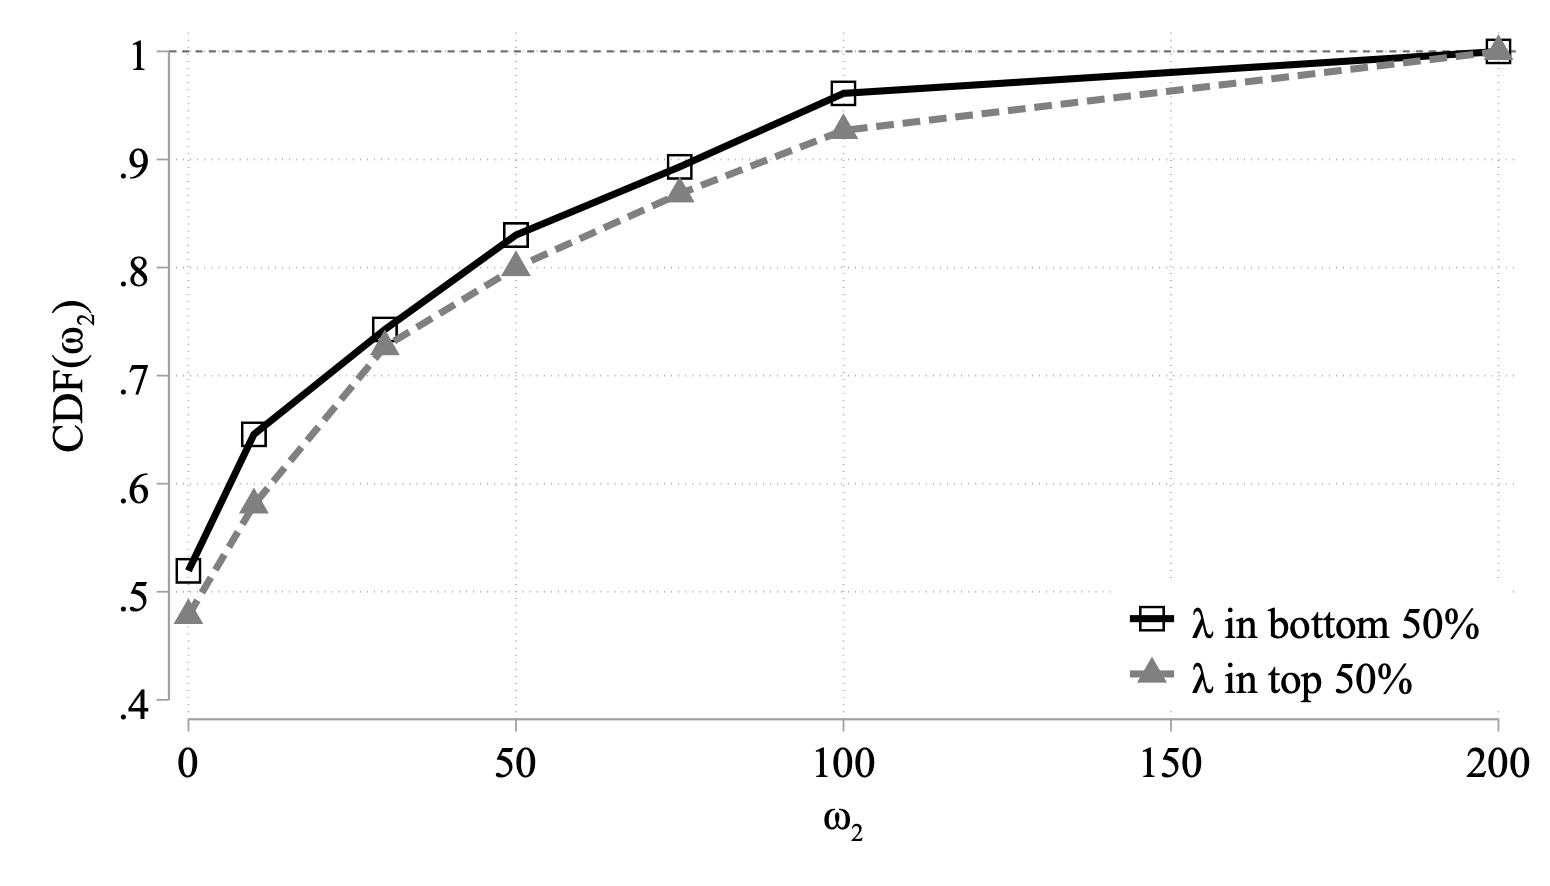
\includegraphics[width=0.7\textwidth]{figures/omega2_cdf_formatted.png}
\caption*{\footnotesize Notes: This Figure plots the CDF of $\omega_{2}$ for districts
with $\lambda_{d}$ above and below the median. The distribution of $\omega
_{2}$ in the first group first-order stochastically dominates that in the
second group, i.e., districts with more low-achieving students are more likely
to reward teacher effectiveness. }
\vspace{-0.7cm}
\end{figure}

To further investigate districts' wage schedule choices, in Table 4 we use OLS
regressions to relate a district's reward for teacher contribution
($\omega_{d2}$) to the following groups of variables: 1) the share of
Democratic votes in the 2012 Presidential election among residents in $d$'s
county $\left(  dem_{d}\right)  \citep{dailykos_statewide_results_2021};$ 2) district $d$'s student body, budget,
capacity, and urbanicity; 3) the characteristics of teachers initially working
in $d$ and in $d$'s commuting zone; and 4) the characteristics of district
$d$'s residents \citep{nces_acs_ed_2013_2017}. In Column (1), we show a
specification that includes the variables in groups 1), 2), and 3). We find
that districts with a larger share of Democratic votes and districts with
larger capacity tend to offer lower rewards for teacher effectiveness, i.e.,
they are more reluctant to deviate from the old zero-reward regime. We also
find that $\omega_{d2}$ is (insignificantly) positively correlated with the
share of low-achieving students in $d$ and with $d$'s budget, while it is
(insignificantly) negatively correlated with the effectiveness of tenured
teachers initially working in $d$. Although insignificant, the negative point
estimate is intuitive: If tenured incumbents, whom the district cannot
dismiss, are ineffective, a district can set higher $\omega_{d_{2}}$ (higher
penalty for low effectiveness) to push these teachers out. In Column (2), we add
controls of the income distribution in the district; in Column (3), we further
control for residents' age and education. Estimates of the coefficient
associated with $dem_{d}$ are robust across specifications. This suggests that
a district's wage schedule choice is explained, to a large extent, by the
political views of its residents.

\begin{table}[ptb]
\caption{Explaining District Reward for Teacher Contribution $\omega_{d2}$
(2014)}
\centering
\begin{tabular}{@{}
    l
    c @{\hspace{1.5em}\extracolsep{\fill}}
    c @{\hspace{1.5em}\extracolsep{\fill}}
    c
@{}}
\hline\hline
& (1) & (2) & (3) \\
\hline
Share Democratic votes ($dem_{d}$, 2012)
& -56.46 (26.39)
& -57.52 (26.43)
& -54.50 (27.12) \\

Capacity
& -0.35 (0.17)
& -0.35 (0.17)
& -0.30 (0.18) \\

$\lambda_{d}$
& 25.24 (24.58)
& 36.56 (28.20)
& 36.62 (31.18) \\

Budget per teacher
& 0.53 (0.46)
& 0.47 (0.48)
& 0.55 (0.48) \\

Avg. TC, incumbent teachers
& 200.4 (2740.2)
& 193.3 (2719.0)
& 306.9 (2708.3) \\

Avg. TC, tenured incumbent teachers
& -508.9 (2749.3)
& -501.8 (2731.4)
& -614.1 (2720.1) \\

Experience/education, incumbent teachers
& Yes & Yes & Yes \\

TC and share tenured, teachers in CZ
& Yes & Yes & Yes \\

District urbanicity
& Yes & Yes & Yes \\

Distribution of residents' income
& No & Yes & Yes \\

Distribution of residents' age/education
& No & No & Yes \\
\hline
$R^{2}$
& 0.06 & 0.06 & 0.06 \\

\# obs.
& \multicolumn{3}{c}{411} \\
\hline\hline
\end{tabular}
% restore default spacing for later tables
\setlength{\tabcolsep}{6pt}

\caption*{ \footnotesize{Notes: OLS estimates of regressions with
$\omega_{d2}$ as the dependent variable. Residents' income is captured by the
natural logarithm of median income, the poverty rate, and the fraction of
households with incomes higher than \$200,000. The distribution of residents'
age and education is captured by the fractions of people younger than 15,
those older than 64, and those with a college education. Robust standard
errors are in parentheses.}}
\vspace{-0.7cm}
\end{table}

\section{Estimation Results}

\subsection{Parameter Estimates}

Table 5 shows estimated model parameters, along with their standard errors (in
parentheses) derived numerically via the Delta Method. Panel A shows estimated
parameters governing teachers' preferences. For most teachers, districts with
higher fractions of low-achieving students $\left(  {\small \lambda}%
_{d}\right)  $ are less desirable: An average teacher puts a premium of about
\$4,100 on a district with ${\small \lambda}_{d}=0.3$ over an otherwise
identical district with ${\small \lambda}_{d^{\prime}}=0.7$. However, teachers
who are more effective in teaching low-achieving students are more willing to
teach in these districts: The coefficient of $c_{1}\times{\small \lambda}_{d}$
is positive, although imprecisely estimated. Rural districts are less
attractive than their urban and suburban counterparts. The remainder of Panel
A shows that teachers face high moving costs, especially among more
experienced teachers.\footnote{Moving rates are consistently higher for less
experienced teachers throughout our simulations. For example, in the baseline
equilibrium, among teachers with $d_{0}\neq0$, the average moving rate by
experience group is 0.71, 0.17, 0.05, 0.001, and 0.001.} Individuals compare
the total value of each option when making their choices, including their
preference shocks (governed by ${\small \sigma}_{\epsilon})$. High moving
costs help explain the\ lack of teacher mobility, especially among more
experienced teachers, while preference shocks absorb idiosyncratic reasons for
mobility. Our findings of large moving cost and dispersion of preference
shocks are consistent with previous studies on worker mobility \citep[e.g.,][]{kennan2011effect}.

\begin{table}[!tb]
\caption{Parameter Estimates}
\centering
{\setlength{\tabcolsep}{8pt}

\begin{tabular}{@{}
    l c c
    @{\hspace{2em}\extracolsep{\fill}}
    l c c
@{}}
\hline\hline
\multicolumn{6}{l}{\textbf{A. Teacher Preferences}}\\
Parameter & estimate & s.e. & Parameter & estimate & s.e. \\
\hline
wage (\$1,000) & 1 (normalized) & -- 
& $I(d \neq d_{0}) \times$Yrs of experience: &  &  \\
$e^{\lambda_{d}}$ & -6.22 & (1.38)
& \multicolumn{1}{l}{1--2} & -10.66 & (6.69) \\

$c_{1} \times \lambda_{d}$ & 22.11 & (26.34)
& \multicolumn{1}{l}{3--4} & -55.23 & (22.03) \\

$q_{d}$: urban & 16.55 & (3.36)
& \multicolumn{1}{l}{5--9} & -78.94 & (6.33) \\

$q_{d}$: suburban & 21.19 & (2.13)
& \multicolumn{1}{l}{10--14} & -150.96 & (41.10) \\

$q_{d}$: large metro & 2.96 & (8.31)
& \multicolumn{1}{l}{$\geq 15$} & -151.29 & (50.26) \\

$\sigma_{\epsilon}$ & 18.73 & (0.94)
& $I(z_{d} \neq z_{d_{0}})$ & -19.98 & (22.86) \\

 &  & 
& $\ln(\text{distance in miles})$ & -14.42 & (5.24) \\
\hline
\multicolumn{6}{l}{\textbf{B. District Preferences}}\\
Parameter & estimate & s.e. & Parameter & estimate & s.e. \\
\hline
$c_{1}$ & 1 (normalized) & -- 
& Yrs of experience: & &  \\
$c_{2}$ & 0.67 & (0.02)
& \multicolumn{1}{l}{1--2} & 0.012 & (0.11) \\

MA or above & $2.0 \times 10^{-5}$ & (0.03)
& \multicolumn{1}{l}{3--4} & 0.016 & (0.02) \\

& & 
& \multicolumn{1}{l}{5--9} & 0.017 & (0.37) \\

&  & 
& \multicolumn{1}{l}{10--14} & 0.033 & (0.02) \\

&  & 
& \multicolumn{1}{l}{$\geq 15$} & 0.040 & (0.03) \\
\hline\hline
\end{tabular}
}

\caption*{ \footnotesize{Notes: Model parameter estimates. Standard errors
(in parentheses) are calculated numerically via the Delta Method.}}
\vspace{-0.7cm}
\end{table}

Panel B shows district preference estimates. Districts significantly value a
teacher's contribution to its students' achievement but do not value teacher
experience and education per se. In addition, districts value a teacher's
contribution to its low-achieving students more than their contribution to its
high-achieving students. Table A1 shows the estimated parameters governing the
cost a district faces for deviating from the pre-Act 10 wage schedule;
consistent with Table 4, the estimates indicate that districts with a larger
share of democratic voters face a higher cost. In Section \ref{mag}, we
explore the implications of both teachers' moving costs and districts' costs
for deviating from rigid wage schedules.

\subsection{Model Fit\label{within fit}}

We present within-sample fits in the main text and the model validation exercise in Appendix B7. Table \ref{tab:modelfit_aux12} shows that the model well captures the
teacher-school sorting as summarized by the two regressions specified in
Section \ref{aux} (Aux 1a on the left and Aux 1b on the right). The model fits
the data well as measured by Aux 1a but less so as measured by Aux 1b.
Notably, in Aux 1a, the model replicates the strong positive coefficient on
$c_{1}\times\lambda_{d}$ (0.57 in the data vs 0.50 in the model); in Aux 1b,
this coefficient is -0.02 in the data but 0.001 in the model. The upper panel
of Table \ref{tab:modelfit_wage} shows model fits for the distribution of
$\omega.$ Overall, the model fits the data well, although it underpredicts the
dispersion of $\omega_{2}\ $and the fraction of districts choosing $\omega
_{2}=0$. The lower panel shows model fits for district characteristics by
whether or not they reward teacher contribution; these statistics are not
directly targeted in the estimation. Consistent with the data, the model
predicts that districts with $\omega_{2}>0$ are slightly more disadvantaged.
Appendix Tables B21 and B22 show additional model fit measures (Aux 2
and Aux 4), which are also good. 


\section{Counterfactual Experiments}

We use our estimated model to examine the equity-efficiency implication of
flexible pay and to evaluate a set of counterfactual state bonus programs.
Throughout, we measure efficiency and equity in terms of students' access to
effective teachers, which maps into students' achievement.\footnote{Although
teachers make choices to maximize their welfare in each case, we do not
consider teachers' welfare in our efficiency-equity calculations.}
Specifically, we pay special attention to the following metrics:\footnote{More
specifically, letting $\Pr\left(  i\text{ in }d\right)  $ be the probability
that $i$ works in $d,$ the definitions of these metrics are as follows:
$\overline{TC}_{D^{\prime}}=\frac{\sum_{d\in D^{\prime}}\sum_{i}\Pr\left(
i\text{ in }d\right)  {\small TC}\left(  c_{i},\lambda_{d}\right)  }%
{\sum_{d\in D^{\prime}}\sum_{i}\Pr\left(  i\text{ in }d\right)  },$
$\overline{C}_{1}=\frac{\sum_{d}\sum_{i}\Pr\left(  i\text{ in }d\right)
{\small c}_{i1}\lambda_{d}}{\sum_{d}\sum_{i}\Pr\left(  i\text{ in }d\right)
\lambda_{d}},$ and $\overline{C}_{2}=\frac{\sum_{d}\sum_{i}\Pr\left(  i\text{
in }d\right)  {\small c}_{i2}\left(  1-{\small \lambda}_{d}\right)  }{\sum
_{d}\sum_{i}\Pr\left(  i\text{ in }d\right)  \left(  1-{\small \lambda}%
_{d}\right)  }.$} \newline1. Average total contribution $\overline
{TC}_{D^{\prime}}$ among teachers working in a given group of districts
$D^{\prime}\subseteq D$. Since teacher contribution enters student achievement
additively, an increase in $\overline{TC}_{D^{\prime}}$ maps one-to-one into
an increase in the average achievement for students in $D^{\prime}.$ When
$D^{\prime}=D,$ $\overline{TC}_{D}$ measures the overall match
\emph{efficiency} in the market. Moreover, a policy will improve
cross-district educational equity if it increases $\overline{TC}_{D^{\prime}}$
more for high-$\lambda_{d}$ districts, i.e., districts with higher fractions
of low-achieving students, than it does for low-$\lambda_{d}$
districts.\newline2. Average teacher contribution to the state's low-achieving
students $\overline{C}_{1}$ and high-achieving students $\overline{C}_{2}$. An
increase in $\overline{C}_{1}$ ($\overline{C}_{2}$) maps one-to-one into an
increase in the average achievement for low-achieving (high-achieving)
students. A policy will narrow the achievement gap between the two groups if
it improves $\overline{C}_{1}$ more than it improves $\overline{C}_{2}$.

\subsection{Flexible Pay versus Rigid Pay\label{rigid}}

To examine the equity-efficiency implication of a regime switch from rigid pay
to flexible pay, we contrast the baseline flexible-pay equilibrium (as
described in Section \ref{model}) with the counterfactual equilibrium where
all initial conditions are kept the same, but the rigid wage schedule
$\omega=\left(  1,0\right)  $ is imposed on all districts.

\begin{table}
\caption{Flexible Pay vs Rigid Pay}
\centering
{\setlength{\tabcolsep}{10pt}
\begin{tabular}{@{} l c c c @{\hspace{1.2em}} c @{}}
\hline\hline
& \multicolumn{3}{c}{\% difference: $(\text{Flexible} - \text{Rigid})/\lvert \text{Rigid}\rvert$}
& Frac. low-achieving \\\vspace{0.1cm}
\cline{2-4}
& $\overline{TC}$ (all) & $\overline{C}_{1}$ (low-achieving) & $\overline{C}_{2}$ (high-achieving)
& ($\lambda_{d}$) \\
\hline
All Districts & 0.04 & -0.01 & 0.10 & 0.50 (0.12) \\
\hline
\emph{By quartile of $\lambda_{d}$}:& & & & \\ 
\hspace{1em}4th & -0.34 & -0.24 & -0.57 & 0.64 (0.06) \\
\hspace{1em}3rd & 0.37  & 0.45  & 0.25  & 0.54 (0.02) \\
\hspace{1em}2nd & 0.05  & 0.03  & 0.06  & 0.47 (0.02) \\\
\hspace{1em}1st & 0.05  & -0.37 & 0.27  & 0.34 (0.07) \\
\hline\hline
\end{tabular}
}
\caption*{ {\footnotesize {Notes: Columns 1--3 report the percent difference in $\overline{TC}$, $\overline{C}_{1}$, and $\overline{C}_{2}$ between the flexible-pay and rigid-pay regimes. Col. 4 reports the mean (cross-district std. dev.) of the fraction of low-achieving students in each district group.}}}
\vspace{-0.7cm}
\end{table}

The first three columns in Table 6 show percentage changes in $\overline{TC},$
$\overline{C}_{1},$ and $\overline{C}_{2}$ associated with a shift from the
rigid-pay regime to the flexible-pay regime. These effects are shown in Row 1
for the entire state, and in Row 2 to Row 5 for each of the four quartiles of
districts ranked by $\lambda_{d}$ (fraction of low-achieving students) from
the highest to the lowest. The last column summarizes the mean and the
standard deviation of $\lambda_{d}$ among districts in each row. 

The following four findings stand out: 

\noindent (1) Flexible pay allows districts to directly
reward teacher contribution, which encourages comparative advantage-based
sorting and hence improves efficiency: At the state level, teachers' total
contribution $\overline{TC}$ increases by 0.04\%. However, on average, the
gain accrues entirely to high-achieving students, while low-achieving students
experience a slight decline in teacher contribution, widening achievement gap
between the state's two groups of students.

(2) As districts'
competition intensifies under flexible pay, districts in the top quartile of the
fraction of low-achieving students lose by all three metrics, with both types
of students losing effective teachers to other districts. This is because, all
else being equal, most teachers prefer districts with fewer low-achieving
students. 

(3)\ Perhaps surprisingly, districts in the second-highest quartile of $\lambda_{d}$
 gain the most by almost all three metrics. This is largely
explained by teachers' moving costs. To avoid large moving costs, as effective
teachers move out of highest-$\lambda_{d}$ districts, they are more likely to
move to nearby districts, which are less likely to be low-$\lambda_{d}$
districts due to the fact that student bodies tend to be similar among nearby
districts (Appendix Figure B10). In general, teachers' unwillingness to move explains why the equity-efficiency tradeoff between the two pay regimes is quantitatively small.

(4) Flexible pay allows
districts to compete more effectively for teachers better suited for their
students; as a result, a district's majority student group---low- or
high-achieving---benefits more or loses less than the minority group (Column 2
versus Column 3). Most evidently, in districts where a large majority of
students are high-achieving (Row 5), teacher effectiveness improves by 0.27\%
for high-achieving students while\ it decreases by 0.37\% for low-achieving
students, widening the within-district achievement gap between the two groups
of students.

In sum, the impacts shown in Table 6, although small in magnitude, reflect a
trade-off between efficiency and equity. Flexible pay improves efficiency, but
it also widens\ achievement gaps across districts and between low- and
high-achieving students.

\subsection{State-Funded Bonuses}

Given the trade-off reflected in Table 6, we now explore the possibility of
improving \emph{both} efficiency \emph{and} equity under flexible pay via a
commonly used policy tool: state-funded teacher bonuses. To design our bonus
formula, we build on the insights provided by our estimated model. On the
supply side, although teachers differ in their comparative advantages, they
face large moving costs, which act as an obstacle to efficient sorting. In
addition, most teachers prefer teaching high-achieving students, which acts as
an obstacle to equity. On the demand side, a large fraction of districts
choose not to reward teacher effectiveness, which constitutes an additional
obstacle to both efficiency and equity.

Our bonus formula is designed to overcome these obstacles. For the supply
side, the formula consists of an efficiency incentive and an equity incentive;
for the demand side, it gives a direct incentive for districts to reward
effectiveness. Specifically, a teacher with effectiveness $c=\left(
c_{1},c_{2}\right)  $ teaching in district $d\ $would obtain a state-funded
bonus given by
\begin{equation}
B\left(  c,\lambda_{d},\omega_{d}\right)  =\min\left\{  \max\left\{  \left[
r_{0}TC\left(  c,\lambda_{d}\right)  +r_{1}c_{1}\lambda_{d}\right]
\omega_{d2},0\right\}  ,\overline{B}\right\}  . \tag{B}%
\end{equation}
To avoid extreme values, we bound bonuses between $0$ and $\overline{B}$ (set
at twice the standard deviation of the observed wage distribution). Between
the two bounds, the formula has three features that make our formula novel and
distinct from existing teachers' bonus formulae
\citep[see][for reviews]{neal2011design,pham2021teacher}. \newline(1) The
component $r_{0}TC\left(  c,\lambda_{d}\right)  $ rewards a teacher for their
TC at the rate $r_{0}$. Since a teacher's TC is higher\ when their comparative
advantage better matches a district's student composition, this component
incentivizes more efficient sorting.\newline(2) The component $r_{1}%
c_{1}\lambda_{d}$ additionally rewards a teacher for their\ $c_{1}\lambda_{d}$
(contribution to $d$'s low-achieving students) at the rate $r_{1}$. By
providing an additional incentive for high-$c_{1}$ teachers to teach in
low-achievement districts, this component directly favors these districts,
improving equity. The goal of equity is shared by many existing formulae that
reward teachers for working in disadvantaged places
\citep{bobba2021teacher,swain2019selective}; however, designed solely to
improve equity, these formulae do not account for efficiency. In contrast, our
formula accounts for both equity (via $r_{1}c_{1}\lambda_{d}$) and efficiency
(via $r_{0}TC\left(  \cdot\right)  $) .\newline(3) The factor $\omega_{d2}$
ties a teacher's bonus to the rate at which the district rewards teacher
contribution. Since a higher $\omega_{d2}$ would enable district $d$ to obtain
more state bonuses for its teachers, this feature incentivizes districts to
reward teacher effectiveness in their own wage schedule. This
component---missing from existing bonus formulae---proves to be very important
for program effectiveness.\footnote{Without the third feature, i.e., a
teacher's bonus is based on $r_{0}TC\left(  c,\lambda_{d}\right)  +r_{1}%
c_{1}\lambda_{d}$ regardless of $\omega_{d2}$, programs will be much less
effective. For example, if we set $r_{1}=0$ and adjust $r_{0}$ to exhaust the
same total budget of \$1,620 per teacher, this alternative formula will lead
to an efficiency gain of 0.08\%, while our original formula will lead to an
efficiency gain of 0.18\%.}

The key policy variables in our formula are the bonus rates $\left(
r_{0},r_{1}\right)  .$ Different vectors of $(r_{0},r_{1})$ would induce
different reactions from districts and teachers and hence different
equilibrium outcomes.\footnote{We assume that our model parameters are
policy-invariant. In particular, we do not consider the possibility that state
bonuses may directly change voters' supports for teacher unions and wage
rigidity, thereby changing the resistance cost function $R\left(
\cdot\right)  $. In Section 7.2.1 and Appendix B6.3, we examine how
policy effects differ in the absence of resistance costs.} For illustration,
we present results from three bonus programs under flexible pay (labeled as
New1 to New3), each associated with a different $(r_{0},r_{1})$, and contrast
them with the baseline flexible pay equilibrium (labeled as Base); further
details and additional simulation results are reported in Appendix
B6.3. We calibrate the vector of bonus rates such that all programs New1 to
New3 are equally costly in the equilibrium, at about \$1,620 per teacher.
Given this total cost, the equilibrium average state bonus for each recipient
ranges from \$4,120 to \$4,210, depending on program specifics (lower panel of
Table 7). These amounts are comparable to relatively mild bonus programs
implemented in other states, but, as mentioned above, with very different
formulae than ours.\footnote{For example, in 2014 dollars, the per recipient
bonus was between \$1,910 and \$13,370 in the 1989 Tennessee Career Ladder
Evaluation (CLE) program, between \$1,719 and \$3,420 in the 2007 NYC bonus
program, and between \$5,500 and \$16,500 in the 2008 Tennessee POINT program
\citep{neal2011design}. Findings from these programs are mixed. Math scores
improved by 3\% under CLE; the NYC bonus program had no effect on achievement;
and POINT had no effect on achievement except for one grade (the effect was
positive for one year).}

Each of our three programs serves a different policy goal. In \textbf{New1},
we seek to improve efficiency, as measured by total $\overline{{\small TC}}$
at the state level. Among the simulations we have conducted, the vector
$(r_{0},r_{1})=\left(  2.3,3.1\right)  \ $performs the best and improves
efficiency by 0.26\%. It is worth noting that, even though our goal is to
improve efficiency, in New1, teachers receive an additional bonus for their
contribution to low-achieving students ($r_{1}>0$). This is because most
teachers, including many who have a comparative advantage in teaching
low-achieving students, prefer to teach high-achieving students. Therefore,
bonus schemes that favor districts with more low-achieving students outperform
a purely TC-based bonus scheme: At the same total cost, the latter leads to a
lower efficiency gain of 0.18\% (Appendix Table B18). However, the
gains under New1 accrue only to high-achieving students, who gain by 0.59\% on
average, while low-achieving students lose by 0.06\% on average. Similarly,
the gains go to districts serving fewer low-achieving students, at the expense
of districts serving more low-achieving students. In sum, New1 succeeds in its
goal of improving efficiency, but ends up hurting equity.

\begin{table}
\caption{State-Funded Bonuses}
\centering
{\setlength{\tabcolsep}{16pt}

\begin{tabular}{@{}
    l
    @{\extracolsep{\fill}}
    c c c
@{}}
\hline\hline

& \multicolumn{3}{c}{\% from Base: $(\text{New}-\text{Base})/|\text{Base}|$} \\ 
\cline{2-4}

& (1) & (2) & (3) \\

& \shortstack{New1\\(Efficiency)}
& \shortstack{New2\\(Equity)}
& \shortstack{New3\\(Eq.+Eff.)} \\

\hline

$\overline{TC}$ for all students in the state (efficiency)
& 0.26 & 0.04 & 0.15\\

$\overline{C}_{1}$ for low-achieving students in the state
& -0.06 & 0.35 & 0.16\\

$\overline{C}_{2}$ for high-achieving students in the state
& 0.59 & -0.26 & 0.14\\

$\overline{TC}$ in 4th quartile $\lambda_{d}$ districts
& -0.33 & 1.01 & 0.47\\

$\overline{TC}$ in 3rd quartile $\lambda_{d}$ districts
& -0.34 & 0.69 & 0.21\\

$\overline{TC}$ in 2nd quartile $\lambda_{d}$ districts
& 0.41 & 0.27 & 0.32\\

$\overline{TC}$ in 1st quartile $\lambda_{d}$ districts
& 1.08 & -1.37 & -0.27\\

\hline

Bonus rates $(r_{0},r_{1})$
& $(2.3, 3.1)$ & $(0, 7.0)$ & $(1.6, 4.3)$\\

Teachers receiving state bonuses ($B>0$)
& 38.5\% & 39.4\% & 39.0\%\\

Avg. bonus for recipients $E(B\mid B>0)$ (\$1,000)
& 4.21 & 4.12 & 4.15\\

Program cost (\$1,000 per teacher)
& \multicolumn{3}{c}{1.62} \\

\hline\hline

\end{tabular}
}

\caption*{ {\footnotesize {Notes: Flexible-pay equilibrium with different bonus programs.
The top panel shows changes in the metrics described in the text between the
equilibrium with the bonus program and the baseline flexible-pay equilibrium.
The bottom panel summarizes the characteristics of each bonus program. New1 aims at improving efficiency, New2 aims at improving equity, and New3 aims at improving both efficiency and equity.}%
}}
\vspace{-0.7cm}
\end{table}

In an attempt to improve equity, in \textbf{New2} we reward teachers only
based on $c_{1}\lambda_{d}$, thus providing strong incentives for high-$c_{1}$
teachers to teach in districts with more low-achieving students. New2 leads to
a state average gain of 0.35\% for low-achieving students but a 0.26\% loss
for high-achieving students. Cross-district achievement gaps also narrow as
districts serving more low-achieving students gain more from this program.

Results from New1 and New2 illustrate the dilemma often faced by policy
makers: the trade-off between efficiency and equity. Is it possible to gain in
both efficiency and equity in a more balanced manner and benefit both types of
students? Our final program \textbf{New3 }aims at achieving this goal.
Intuitively, the vector of bonus rates in this case should be in between those
under New1 and New2. Indeed, at bonus rates $\left(  r_{0}^{2},r_{1}%
^{2}\right)  =\left(  1.6,4.3\right)  ,$ New3 leads to a 0.15\% efficiency
gain, with low-achieving students gaining slightly more than high-achieving
students. In addition, New3's impacts are also more evenly distributed across
districts than both New1 and New2.

\begin{remark}
For equity, we focus on the achievement gap between the state's low- and
high-achieving students ($\overline{C}_{1}$ versus $\overline{C}_{2}$) and the
achievement gap across districts ($\overline{{\small TC}}$ in high- versus
low-$\lambda_{d}$ districts). A program that improves the average achievement
of a student group or a district group is not guaranteed to benefit all
students in that group. For example, although New2 is designed to benefit
low-achieving students on average, it causes losses for both types of students
in the lowest-$\lambda_{d}$ district group (Appendix Table B18).
Similarly, for efficiency, we focus on the state's average student achievement
(state level $\overline{{\small TC}}$); it is impossible to achieve Pareto
improvement at the student level.
\end{remark}

\subsubsection{Discussion: Magnitudes of Policy Impacts\label{mag}}

Our counterfactual simulations demonstrate that it is possible to design bonus
programs to improve efficiency and equity. In general, these two goals are
hard to achieve simultaneously. For example, Section \ref{rigid} shows that a
flexible pay regime improves efficiency but hurts equity. Our contribution is
to show that, by exploiting teachers' comparative advantages, \emph{carefully
designed} policies can lead the market equilibrium toward more efficient and
equitable allocations. However, the magnitudes of our counterfactual policy
impacts are small, consistent with previous studies on the limited impacts of
monetary incentives on teacher sorting
\citep[e.g.,][]{clotfelter2011teacher,russell2020ects}. We now investigate
some possible reasons.

One possible reason is that the current equilibrium teacher-school sorting is
close to being efficient and/or equal, so there is not much room for
improvement. This is not the case in our data: Appendix B6.1 shows that
it is possible to achieve much higher efficiency or equity if one could ignore
teachers' preferences and dictatorially allocate teachers to districts. An
efficiency-seeking dictator can improve efficiency by 31\% relative to the
baseline (at the cost of equity); a dictator who seeks to help low-achieving
students can improve their performance by 70\% (while hurting high-achieving
students by 56\%).

In reality, though, a feasible policy intervention needs to respect teachers'
and districts' preferences and constraints, which ultimately govern
equilibrium outcomes and policy effects. We quantify the impact of two
potentially important factors: teachers' moving costs $\Gamma\left(
\cdot\right)  $ and districts' resistance costs $R\left(  \cdot\right)  $. To
do so, we consider the following two counterfactual cases. \newline Case 1:
Teachers have zero moving costs, i.e., $\Gamma\left(  \cdot\right)
=0$.\newline Case 2: In addition to $\Gamma\left(  \cdot\right)  =0,$
districts face zero resistance costs, i.e., $R\left(  \cdot\right)
=0$.\newline For each of these cases, we simulate the new flexible-pay
equilibrium and compare it with the baseline flexible-pay equilibrium.

The results are shown in the first two columns of Table 8. Relative to the
baseline, teacher TC is 2.43\% higher in the equilibrium without moving costs
(Column 1). This comes at the cost of equity: Average TC declines by 6.28\%
for low-achieving students and increases by 10.78\% for high-achieving
students. These changes are larger than the impact of any of our bonus
programs shown in Table 7. This is unsurprising since teachers' moving costs
(Table 5) are much higher than our bonuses. When we additionally remove
districts' resistance costs (Column 2), TC increases further and equity
worsens.\footnote{By setting both the moving cost and the resistance cost to
zero, Case 2 can provide a sense of the long-run equilibrium outcomes under
flexible pay, when the market has fully adjusted to a new steady state. We
thank an anonymous referee for pointing this out.}

\begin{table}
\caption{Moving Costs, Resistance Costs, and Policy
Impacts}
\centering
{\small
\begin{tabular*}{\textwidth}{@{\extracolsep{\fill}} l c c c c @{}}
\hline\hline

& \multicolumn{4}{c}{\% change between scenarios $S'$ vs $S$: $(S'-S)/|S|$} \\
\cline{2-5}

& (1) & (2) & (3) & (4) \\

& Case 1 vs Base
& Case 2 vs Base
& Case 2 New2 vs Case 2
& New2 vs Base \\

\hline

$\overline{TC}$ & 2.43 & 2.72 & 0.05 & 0.04\\
$\overline{C}_{1}$ & -6.28 & -7.01 & 1.86 & 0.35\\
$\overline{C}_{2}$ & 10.78 & 12.05 & -1.41 & -0.26\\

\hline\hline
\end{tabular*}
}
\caption*{{\footnotesize {Notes: Differences in TC, $c_{1}$, and $c_{2}$, between the baseline
flexible-pay equilibrium and equilibria under different scenarios. \emph{Base}
refers to the baseline flexible-pay equilibrium. \emph{Case 1} refers to
flexible-pay equilibrium with zero moving cost. \emph{Case 2 } refers to
flexible-pay equilibrium with zero moving cost and zero resistance costs. \emph{New2} aims at improving equity.}%
}}
\vspace{-0.7cm}
\end{table}

The results above suggest that teachers' moving costs are a major obstacle for
efficiency, but in their absence the achievement gap between low- and
high-achieving students would be larger. Districts' resistance costs for
deviating from rigid pay mildly enhance these effects. These two costs could
also play a major role in mediating the impact of our counterfactual bonus
programs. To illustrate this, we introduce our bonus program \textbf{New2} to
the market under Case 2. Recall that New2 seeks to help low-achieving students
by rewarding teachers only based on $c_{1}\lambda_{d};$ we re-calibrated bonus
rates to keep the total cost the same as before. We find that the impact of
New2 is larger on an economy without moving and resistance costs (Column 3)
than it is on the baseline economy (Column 4).\ Without resistance costs,
districts are more willing to reward teacher contribution; without moving
costs, teachers are more willing to move. As a result, New2 increases
low-achieving students by 1.86\% without moving and resistance costs, but only
by 0.35\% when these costs are present. Taken together, our results imply that
the effectiveness of teacher bonus schemes hinges on teachers' willingness to
move, districts' willingness to change their wage schedules, and the
interaction of these two factors.

\subsection{Additional Simulations}

We have conducted additional simulations in Appendix B6, the results of
which are summarized below.

\paragraph{Extensive Margin Responses and Repeated Static Games}

As discussed in Section \ref{discuss}, our framework is static and it
abstracts from teachers' entry and exit decisions. As such, our policy
implications are best interpreted as short-run effects. A rigorous analysis of
policy impacts in the long run with teachers' extensive-margin responses is
beyond the scope of our paper. As an attempt to understand the impact of state
bonus programs when teachers' entries and exits are taken into account, we
conduct additional simulations in a static setting and in a setting where the
static game is played repeatedly over time. To conduct these exercises, we
need to make additional assumptions. With these assumptions, we first estimate
teachers' entry and exit probabilities in the baseline equilibrium. This
procedure estimates these baseline probabilities as functions of teachers'
observables including $\left(  c_{1},c_{2}\right)  ,$ but it does not allow us
to estimate how these probabilities would change with respect to pay.
Therefore, we borrow extensive-margin elasticities from the literature. With
due caveats, the results from these simulations suggest that if teachers'
extensive-margin responses are non-trivial and if the programs are in place
for multiple years, the equity-efficiency gains from our bonus programs could
be significantly larger. For example, assuming that teachers' entry-exit
elasticity with respect to pay is one and that the static market equilibrium
is played repeatedly for 5 years under a given bonus program, we simulate a
teacher's path of movements at both the extensive margin (entry/exit) and the
intensive margin (the history of districts they work in during these 5 years).
Five years later, our program New1 (New2) would lead to an efficiency gain of
2.99\% (2.08\%) and benefit both low- and high-achieving students.

\paragraph{Program Generosity}

To illustrate the role of program generosity, we simulate three bonus programs
with bonus rates $\left(  r_{0},r_{1}\right)  $ set at 1.5, 2.0, and 2.5 times
$(2.3,3.1),$ the latter being the bonus rates used in New1. These three
programs are increasingly more costly for the state and they all lead to
higher efficiency gains than the gain achieved by New1 (0.26\%). However, the
program effect levels off quickly: The efficiency gain under these three
programs are 0.32\%, 0.34\%, and 0.34\% respectively. This result demonstrates
that with equilibrium responses from both sides of the market, one should not
expect a simple linear relationship between program costs and their impacts.
As such, the design of the bonus program is at least as important as the bonus budget.

\paragraph{The Role of $R\left(  \cdot\right)  $}

To study the role of districts' resistance cost $R\left(  \cdot\right)  $ by
itself, we re-simulated all our three bonus programs by setting $R\left(
\cdot\right)  =0$ while keeping all other parameters at their estimated
values. Perhaps not surprisingly, without resistance costs, districts are more
responsive to our bonus programs. For example, at New1's bonus rates
$(2.3,3.1),$ if we set $R\left(  \cdot\right)  =0,$ this program will yield an
efficiency gain of 0.34\% rather than 0.26\%, but it will also be twice as
costly as New1 with resistance costs.

\section{Conclusion}

Proper allocation of public servants across local employers can have important
implications for both efficiency and equity, but it is difficult to achieve
due to various institutional frictions such as wage rigidity. We study the
equity-efficiency implication of wage rigidity through the lens of the labor
market for public school teachers. To that end, we have developed an
equilibrium model of the teachers' labor market, where teachers differ in
their comparative advantages in teaching low- and high-achieving students and
districts compete for teachers using both wage and hiring strategies. We have
estimated the model using data from Wisconsin following a reform that gave
districts control over teacher pay. %We have validated the model using the pre-reform data under rigid pay.

Our estimated model implies that, ceteris paribus, giving districts control
over teacher pay would lead to more efficient but also more unequal sorting of
teachers across districts. Efficiency improves because districts are allowed
to directly reward teacher contribution, which encourages comparative
advantage-based sorting. Inequality is enlarged because, all else equal,
(most) teachers prefer working in districts with more high-achieving students
and flexible pay makes it even easier for these districts to attract teachers.
We have further demonstrated that, under flexible pay, carefully designed
interventions can improve both equity and efficiency. However, the
effectiveness of these policy interventions and the efficiency-equity comparison across pay regimes hinge on teachers' willingness to
move and districts' willingness to change their wage schedules.

Our analysis abstracts from several important aspects of the teachers' market;
extending our framework along these lines is worth pursuing. The first
extension, which requires additional data, is to incorporate decisions by the
private education sector and to consider the competition not only among public
school districts, but also between public and private sectors. The second
extension is to incorporate household sorting
\citep[e.g.,][]{epple1999estimating,epple2003neighborhood,ferreyra2007estimating,epple2008school}.
A third extension is to add teachers' effort choices into our framework. Since
our model takes teacher effectiveness as pre-determined, the efficiency gains
we have found are likely to understate the total effect of our counterfactual
policy intervention. For example, \citet{barlevy2012pay} show that
\textquotedblleft pay for percentile\textquotedblright\ can induce teachers to
allocate socially optimal levels of effort. Finally, our static equilibrium
model is better suited to study short-run rather than long-run policy impacts;
an important but rather difficult extension is to consider the market in a
dynamic equilibrium setting. On the supply side,\ this extension would reflect
teachers' life-cycle concerns; on the demand side, districts would consider
how their choices would affect both their current return and their future
competitiveness.\ Ultimately, this extension would allow for the investigation
of long-run policy impacts.

\singlespacing
\bibliographystyle{chicago}
\bibliography{biblio_wicomp}





\begin{center}
\textbf{{\Large Appendix}}\bigskip
\end{center}

\setcounter{table}{0} \setcounter{figure}{0} \setcounter{section}{0}
\renewcommand{\thesection}{A\arabic{section}}
\renewcommand{\thetable}{A\MakeUppercase{\arabic{table}}} \renewcommand{\thefigure}{A\MakeUppercase{\arabic{figure}}}

\textbf{A1. Districts' Optimal Decisions}

Given $\omega$, district $d$'s job offers $o_{d}\left(  x,c,d_{0}%
|\omega\right)  \in\left\{  0,1\right\}  $ solve the following
problem:\newline$\pi_{d}\left(  \omega\right)  =$
\begin{align}
&  \max_{\left\{  o_{d}\left(  \cdot\right)  \right\}  }\left\{  \int
o_{d}\left(  x,c,d_{0}|\omega\right)  h_{d}\left(  x,c,d_{0},\omega\right)
\left[  xb_{0}+b_{1}\lambda_{d}c_{1}+b_{2}\left(  1-\lambda_{d}\right)
c_{2}\right]  dF\left(  x,c,d_{0}\right)  \right\} \\
s.t.  &  \int o_{d}\left(  x,c,d_{0}|\omega\right)  h_{d}\left(
x,c,d_{0},\omega\right)  dF\left(  x,c,d_{0}\right)  \leq\kappa_{d}%
,\nonumber\\
&  \int o_{d}\left(  x,c,d_{0}|\omega\right)  h_{d}\left(  x,c,d_{0}%
,\omega\right)  w_{d}\left(  x,c|\omega\right)  dF\left(  x,c,d_{0}\right)
\leq M_{d}\nonumber\\
&  o_{d}\left(  x,c,d_{0}|\omega\right)  =1\text{ if }x_{1}\geq3\text{ and
}d_{0}=d.\nonumber
\end{align}
Letting $\varphi\left(  x,c,\lambda_{d}\right)  \equiv\left[  xb_{0}%
+b_{1}\lambda_{d}c_{1}+b_{2}\left(  1-\lambda_{d}\right)  c_{2}\right]  $, the
first-order condition is%
\[
\varphi\left(  x,c,\lambda_{d}\right)  -\nu_{\kappa}-w_{d}\left(
x,c|\omega\right)  \nu_{M}=0,
\]
where $\nu_{\kappa}$ and $\nu_{M}$ are the non-negative multipliers associated
with the adjusted capacity and budget constraints. The capacity (budget) is
adjusted by netting out the expected slots (wages) filled by tenured incumbent
teachers ($x_{1}\geq3$ and $d_{0}=d)$, for whom $o_{d}\left(  x,c,d_{0}%
\right)  $ has to be $1.$

If the district makes an offer to $\left(  x,c\right)  $ and the offer is
accepted, the district must surrender a slot from its limited capacity and pay
the wage $w_{d}\left(  x,c|\omega\right)  $, inducing the marginal cost
$\nu_{\kappa}+w_{d}\left(  x,c|\omega\right)  \nu_{M}$. Balancing between the
marginal benefit and the marginal cost, the solution is:%

\begin{equation}
o_{d}\left(  x,c,d_{0}|\omega\right)  \left\{
\begin{array}
[c]{l}%
=1\text{ \ \ \ \ if }\varphi\left(  x,c,\lambda_{d}\right)  -\nu_{\kappa
}-w_{d}\left(  x,c|\omega\right)  \nu_{M}>0\\
=0\text{ \ \ \ \ if }\varphi\left(  x,c,\lambda_{d}\right)  -\nu_{\kappa
}-w_{d}\left(  x,c|\omega\right)  \nu_{M}<0\\
\in\lbrack0,1]\text{ if }\varphi\left(  x,c,\lambda_{d}\right)  -\nu_{\kappa
}-w_{d}\left(  x,c|\omega\right)  \nu_{M}=0
\end{array}
\right.  , \label{o}%
\end{equation}%
\begin{equation}
\int o_{d}\left(  x,c,d_{0}|\omega\right)  h_{d}\left(  x,c,d_{0}%
|\omega\right)  dF\left(  x,c,d_{0}\right)  \leq\kappa_{d}, \label{c2}%
\end{equation}%
\begin{equation}
\text{and}\int o_{d}\left(  x,c,d_{0}|\omega\right)  h_{d}\left(
x,c,d_{0}|\omega\right)  w_{d}\left(  x,c|\omega\right)  dF\left(
x,c,d_{0}\right)  \leq M_{d}. \label{c1}%
\end{equation}
Notice that $d_{0}$ affects the optimal job offer decision $o_{d}\left(
x,c,d_{0}|\omega\right)  $ only up to tenured incumbent teachers; for other
teachers, $o_{d}\left(  x,c,d_{0}|\omega\right)  $ is independent from
$d_{0},$ as seen in $\left(  \ref{o}\right)  $.

For a given $\omega,$ a district's job offer decision can be derived by the
following procedure. \newline1) Set $o_{d}\left(  x,c,d_{0}|\omega\right)  =1$
for teachers with $x_{1}\geq3$ and $d_{0}=d.$\newline2) Guess $\nu_{M},$ rank
other teachers by $\varphi\left(  x,c,\lambda_{d}\right)  -w_{d}\left(
x,c|\omega\right)  \nu_{M}.$\newline3) Give offers to teachers from the
top-ranked downwards, until the expected capacity or budget is filled, i.e.,
$\left(  \ref{c2}\right)  $ or $\left(  \ref{c1}\right)  $ is binding.\newline%
4) Calculate the district's value associated with this $\nu_{M},$ and optimize
over $\nu_{M}$ to find the maximum; $o_{d}\left(  \cdot|\omega\right)  $
associated with the optimal $\nu_{M}$ are the optimal job offers under
$\omega.$\ \newline In the outer loop, the district searches over $\omega$ to
optimize its objective $\left(  \ref{pp}\right)  .$ Both $\left(
\ref{c2}\right)  $ and $\left(  \ref{c1}\right)  $ bind in the equilibrium
throughout our simulations.

\bigskip

\textbf{A2. Detailed Function Forms:}

We model the resistance cost a district faces $R_{d}\left(  \omega\right)  $
as the following \newline$R_{d}\left(  \omega\right)  =R\left(  \omega
,dem_{d}\right)  =$%
\begin{equation}
\exp\left(  \xi_{00}+\xi_{01}dem_{d}\right)  +\exp\left(  \xi_{11}+\xi
_{12}dem_{d}\right)  \left\vert \omega_{1}-1\right\vert +\exp\left(  \xi
_{21}+\xi_{22}dem_{d}\right)  \frac{\omega_{2}}{100}. \label{R}%
\end{equation}
The vector $\xi_{0}\equiv\left(  \xi_{00},\xi_{01}\right)  $ captures the
fixed cost of deviating from the rigid-pay schedule; $\xi_{1}$ and $\xi_{2}$
capture the incremental costs for larger deviations from the pre-reform
$\omega_{1}$ and $\omega_{2}$ respectively. Parameters $\left\{  \xi
_{k1}\right\}  _{k=0}^{2}$ measure the extent to which these costs vary with
the political views of district residents, as measured by $dem_{d}.$ To impose
the restriction that costs are non-negative, we use exponential function to
parameterize each of the three parts of the cost but parameters $\xi$
unrestricted.\footnote{We experiemented with different specifications (e.g.,
linear rather than log cost with respect to $\omega_{2}$ deviation), the
current specification fits the data pattern the best.} Estimates of these
parameters are reported in Table A1.

\begin{table}[tbh]
\caption{Other Parameter Estimates: Wage Setting Cost $R\left(  \omega
,dem_{d}\right)  $}%
\label{tab:modelfit_aux12}
\centering
\begin{tabular}
{wl{18em}wc{4em}wc{4em}wc{4em}wc{4em}wc{4em}wc{4em}}\hline\hline
& \multicolumn{3}{c}{constant} &
\multicolumn{3}{c}{$dem_{d}$}\\\cline{2-4}\cline{5-7}
Fixed cost for deviation & $\xi_{00}$ & -0.48 &
(0.20) & $\xi_{01}$ & 1.51 & (0.45)\\
Incremental cost wrt $\omega_{1}$ deviation & $\xi_{10}$ &
1.71 & (0.13) & $\xi_{11}$ & 2.48 &
(0.30)\\
Incremental cost wrt $\omega_{2}$ deviation & $\xi_{20}$ &
-1.00 & (0.10) & $\xi_{21}$ & 2.07 &
(0.34)\\\hline
std dev of $\omega$ choice shocks $\left(\sigma_{\eta_{\omega}}\right)$
& \multicolumn{6}{c}{0.91 (0.03)}\\\hline\hline
\end{tabular}
\caption*{\footnotesize{Notes: Estimates of the parameters in (\ref{R}).
Standard errors (in parentheses) are derived numerically via the Delta
Method.}}
\vspace{-0.7cm}
\end{table}\bigskip

\begin{table}[tbh]
\caption{Model Fit: OLS of Teacher-District Match (post-Act 10)}%
\label{tab:modelfit_aux12}
\centering
\begin{tabular}
{wl{12em}wc{4em}wc{4em}wc{4em}wc{4em}}\hline\hline
Teacher's Choice Set &  \multicolumn{2}{c}{Inferred Offer Set} &
\multicolumn{2}{c}{All Districts} \\
\cline{2-3}\cline{4-5}
& Data & Model & Data & Model \\\hline
wage & 0.001 & 0.001  & -1.5$\times$10$^{5}$ & -0.5$\times$10$^{-5}$\\
$e_{d}^{\lambda}$ &  -0.002 & -0.002 &  -0.0001 & -0.0002\\
$c_{1}\times\lambda_{d}$ & 0.568 & 0.499 &  -0.020 & 0.001\\
$d\neq d_{0}$ &  -0.826 & -0.896 &  -0.982 & -0.998\\
$d\neq d_{0}\times \text{exp}\in[1,2]$ & 0.476 & 0.339 &  0.833 & 0.728\\
$d\neq d_{0}\times \text{exp}\in[3,4]$ & 0.267 & 0.203 &  0.236 & 0.177\\
$d\neq d_{0}\times \text{exp}\in[5,9]$ & 0.085 & 0.078 &  0.099 & 0.057\\
$d\neq d_{0}\times \text{exp}\in[10,14]$ & 0.020 & 0.010 &  0.014 & -0.0002\\
$z_{d}\neq z_{d_{0}}$ &  -0.027 & -0.029 & -0.0004 & -0.0003\\
$\ln(\text{distance})$ &  -0.019 & -0.010 & -0.0001 & 0.00005\\
$q_{d}$: urban & 0.014 & -0.002 &  0.004 & 0.001\\
$q_{d}$: suburban & 0.011 & 0.01 &  0.001 & 0.001\\
$q_{d}$: large metro & 0.096 & 0.127 &  0.012 & 0.001\\\hline\hline
\end{tabular}
\caption*{ \footnotesize{Notes: OLS estimates of equations Aux 1a
(\emph{Inferred Offer set}) and Aux 1b (\emph{All Districts}), obtained
controlling for teacher fixed effects, obtained using the data and the model.
Data are from post-Act 10.}}
\vspace{-0.7cm}
\end{table}\bigskip

\begin{table}[tbh]
\caption{Model Fit: District Wage Schedules}%
\label{tab:modelfit_wage}
\centering
\begin{tabular}
{wl{15em}wc{4em}wc{4em}wc{2em}wc{4em}wc{4em}wc{4em}}%
\hline\hline
\multicolumn{6}{l}{\textbf{A. Summary Stats $(\omega_{1},\omega_{2})$ }} \\
Parameter & 
Data & Model & & Parameter & Data & Model\\\hline
$E(\omega_{1})$ & 0.99 & 0.99 & & 
\multicolumn{1}{l}{$E(\omega_{2})$} & 31.3 & 31.2\\
$E(\omega_{1}^{2})$ & 0.98 & 0.99 & & 
\multicolumn{1}{l}{$E(\omega_{2}^{2})$} & 3562.2 & 3194.1\\
$E(\omega_{1}\omega_{2})$ & 30.47 & 30.87 & & 
\multicolumn{1}{l}{} &  & \\
Fr$\big((\omega_{1},\omega_{2})=(1,0)\big)$ & 0.24 & 0.31 & & 
Fr$(\omega_{2}=0)$ & 0.50 & 0.42\\\hline
\multicolumn{6}{l}{\textbf{B. District Characteristics by $\omega_{2}$ }} \\
&
\multicolumn{2}{c}{$\omega_{2}=0$} &  & & 
\multicolumn{2}{c}{$\omega_{2}>0$}\\
\cline{2-3}\cline{6-7}
& Data & Model &  & &  Data & Model\\
\cline{2-3}\cline{6-7}
Rural & 0.80 & 0.80 &  & &  0.83 & 0.82\\
$\lambda_{d}>\text{median}$ & 0.48 & 0.49 &  & & 
0.52 & 0.50\\
Budget/Capacity (\$1,000) & 51.2 & 51.0 &  & & 
50.7 & 50.9\\\hline\hline
\end{tabular}

\caption*{\footnotesize {Notes: Summary stats of ($\omega_{1},\omega_{2}$)
and district characteristics by $\omega_{2}$: data vs model, post-Act 10.}}
\vspace{-0.7cm}
\end{table}




\end{document}